%    minted language=cpp,

%%%%%%
%%%%%%%%%%%%%%%%%%%%%%%%%%%%%% Title Page Info %%%%%%%%%%%%%%%%%%%%%%%%%%%%%%%%%%%%%%%%%%%
%%%%%%%%%%%%%%%%%%%%%%%%%%%%%%%%%%%%%%%%%%%%%%%%%%%%%%%%%%%%%%%%%%%%%%%%%%%%%%%%%%%%%%%%%%

\documentclass[aspectratio=169,compress]{beamer}
\mode<presentation> 

\usetheme{Warsaw}
\usecolortheme[rgb={0.93,0.03,0.02}]{structure}


\usepackage[algosection,lined]{algorithm2e}
\usepackage{minted}
\usepackage{tcolorbox}
\tcbuselibrary{minted}


% define
%\usepackage{beamerouterthememiniframes} % Para los puntitos 
\setbeamertemplate{footline}[frame number]{}

% include packages
\usepackage{subfigure}
\usepackage{multicol}
\usepackage{amsmath}
\usepackage{epsfig}
\usepackage{graphicx}
\usepackage[all,knot]{xy}
\usepackage{algorithmic}
\xyoption{arc}
\usepackage{url}
\usepackage{multimedia}
\usepackage{hyperref}
\usepackage{tikz}

\usepackage{pgfpages}
\setbeameroption{hide notes} % Only slides
%\setbeameroption{show only notes} % Only notes
%\setbeameroption{show notes on second screen=right} % Both




%\title{20 proyectos de la línea de sistemas inteligentes de la maestría en ingeniería de la UPV: aplicaciones en el área de salud, agroindustria, seguridad y educación}
%\title{Proyectos selectos de visión por computadora y aprendizaje automático del Laboratorio de Sistemas Inteligentes de la UPV} % TecMTY
%\title{Fundamentos de VR-AR mediante aplicaciones Gráficas 3D en Android utilizando OpenGL- Parte I\\ \large 3er Foro Nacional de Tecnologías de la Información y Sistemas Computacionales} % UPP
%\title{Aplicaciones de Realidad Aumentada y Realidad Virtual de la Universidad Polit\'ecnica de Victoria} % UPP
\title{Taller: Recorridos Virtuales de Sitios de Interés de Ciudad Victoria} % UPP

\author{Dr. Marco Aurelio Nu\~no Maganda,\\Ing. Hestybalyz Jackelyn Fernández Cantú,\\
Ing. Ángela Marisol Meléndez Fuentes}
\institute{Universidad Politécnica de Victoria\\ Laboratorio de Sistemas Inteligentes /Maestría en Ingeniería  \\
mnunom@upv.edu.mx  \vspace{.25cm} }

\date{Octubre de 2026}
%\textbf{nmaganda@ccc.inaoep.mx}

%%%%%%%%%%%%%%%%%%%%%%%%%%%%%%%%%%%%%%%%%%%%%%%%%%%%%%%%%%%%%%%%%%%%%%%%%%%%%%%%%%%%%%%%%%
%%%%%%%%%%%%%%%%%%%%%%%%%%%%%% Begin Your Document %%%%%%%%%%%%%%%%%%%%%%%%%%%%%%%%%%%%%%%
%%%%%%%%%%%%%%%%%%%%%%%%%%%%%%%%%%%%%%%%%%%%%%%%%%%%%%%%%%%%%%%%%%%%%%%%%%%%%%%%%%%%%%%%%%

 

%\usepackage[backend=biber,maxcitenames=50,maxbibnames=50,sorting=ydmdddnt]{biblatex}
\usepackage[backend=biber,maxcitenames=50,maxbibnames=50,sorting=none]{biblatex}






%\renewrobustcmd{\mkbibfootnote}{\normalsize\footnotemark\footnotetext}
\setbeamerfont{footnote}{size=\tiny}






\newcommand{\ArchivoPrincipal}{Todos}
\newcommand{\ArchivoSecundario}{Bibliografia}


%Append keywords to identify different bibliography entries.
\DeclareSourcemap{
  \maps[datatype=bibtex, overwrite]{
    \map{
      \perdatasource{\ArchivoPrincipal.bib}
      \step[fieldset=KEYWORDS, fieldvalue=primary, append]
    }
    \map{
      \perdatasource{\ArchivoSecundario.bib}
      \step[fieldset=KEYWORDS, fieldvalue=secundary, append]
    }    
  }
}


\addbibresource{\ArchivoPrincipal.bib}
\addbibresource{\ArchivoSecundario.bib}

\usepackage{listings}
 
% \AtBeginSection[]
%{
%    \begin{frame}
%        \frametitle{Outline}
%        \tableofcontents[currentsection]
%    \end{frame}
%}

\makeatletter
\def\@makefnmark{}
\makeatletter
\setbeamertemplate{footnote}{%
  \parindent 1em\noindent
  \raggedright
  *  
  \insertfootnotetext\par
}



\begin{document}

\frame{
	%\titlepage 
	\begin{titlepage}
	\end{titlepage}
	
}



%\frame{
%\frametitle{Contenido}
%\tableofcontents
%}

\section[RV]{Conceptos de Realidad Virtual}




\begin{frame}{¿Que es la realidad virtual?}


La \textbf{Realidad Virtual} (RV) es un entorno de escenas y objetos simulados por computadora que genera en el usuario la sensación de estar inmerso en él.
\begin{columns}
        \column{0.6\textwidth}
Características principales:
\begin{itemize}
\item \scriptsize Inmersión total: Aíslan el mundo real mediante visores especiales.
\item \scriptsize  Interactividad: Permite interactuar con objetos virtuales en tiempo real.
\item Estímulos sensoriales: Utiliza pantallas, audio 3D y sensores de movimiento.
\item Perspectiva en 3D: El entorno cambia según giras o mueves la cabeza
\end{itemize}

Componentes básicos:
\begin{itemize}
\item \scriptsize El Visor (HMD): Casco con pantallas que cubren todo el campo visual.
\item Controles manuales: Rastrean tus manos para tocar o sujetar objetos interactivos.
\item Sensores de posición: Cámaras o giroscopios que miden tus movimientos físicos. 
\end{itemize}

        \column{0.38\textwidth}
        \begin{center}
        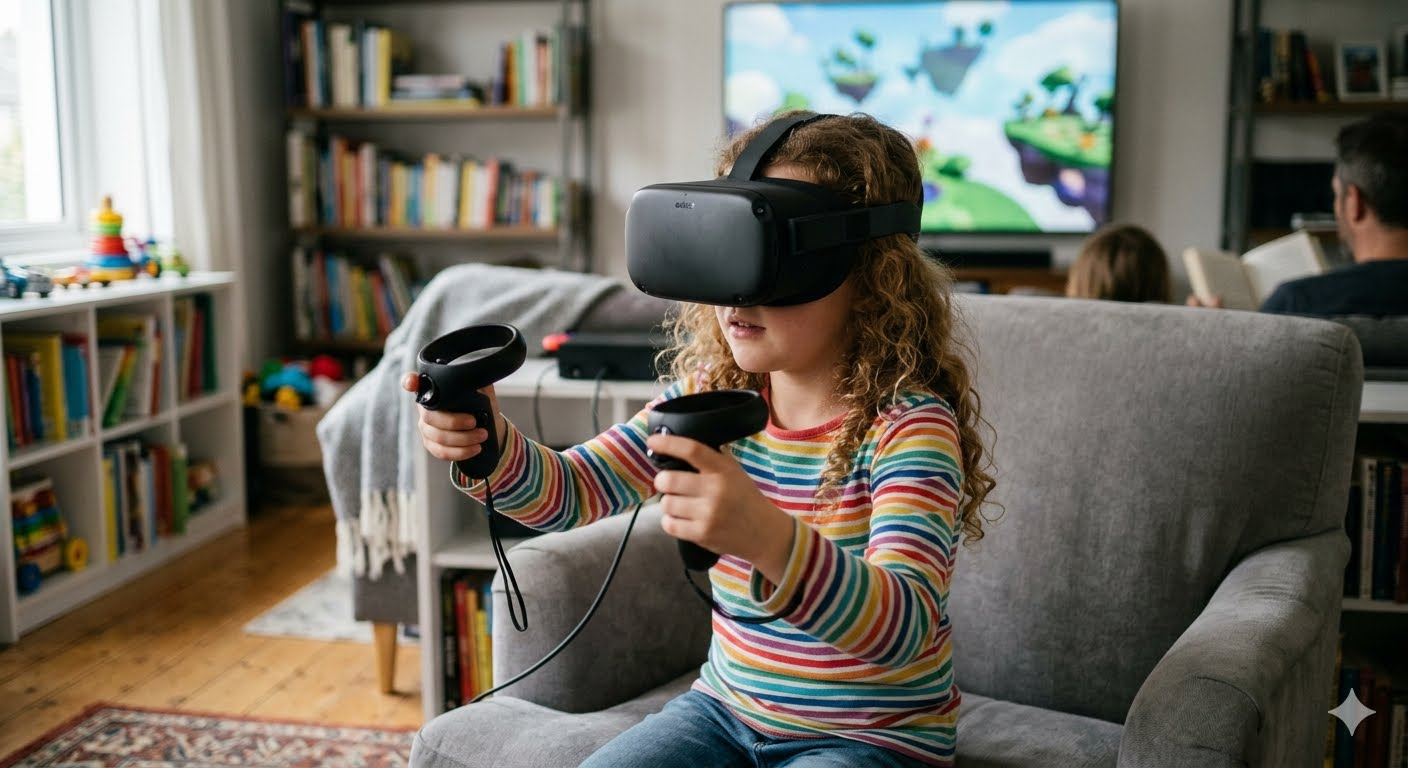
\includegraphics[width=\linewidth]{00_Intro_VR/VR_user.jpeg}
        \end{center}
    \begin{center}
            \tiny Image generated by AI assistant (Gemini AI) based on the prompt by Marco Aurelio Nuño-Maganda, May 28th, 2026.
        \end{center}
\end{columns}

\end{frame}

 



\begin{frame}{Experimento de la Salchicha flotante}

\begin{columns}
        \column{0.6\textwidth}

\textbf{Pasos a seguir: }
\begin{itemize}
    \item Posición inicial: Levanta tus dedos índices y apunta el uno hacia el otro, manteniendo las yemas muy cerca (pero sin que lleguen a tocarse).
    \item Acerca a tu cara: Coloca tus manos a unos 15 o 20 centímetros de tu nariz.
    \item Cambia el enfoque: No mires directamente a tus dedos. Abre bien los ojos y dirige tu mirada a través de ellos, como si estuvieras viendo un objeto lejano al fondo de la habitación.
    \item Observa la ilusión: Al desenfocar tus ojos de los dedos, verás aparecer una pequeña salchicha flotando en el espacio intermedio.
\end{itemize}

        \column{0.4\textwidth}
\begin{center}
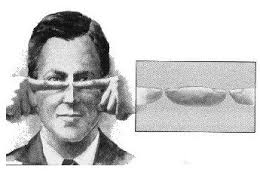
\includegraphics[width=\linewidth]{00_Intro_VR/SalchichaFlotante.jpeg}
\end{center}
\end{columns}

\end{frame}

%\begin{frame}{Experimento de la Salchicha flotante (2)}
%\textbf{¿Que explicación tiene la Salchicha flotante?}
%\begin{itemize}
%    \item El fenómeno ocurre gracias a la visión binocular y el campo visual.
%    \item Cada uno de tus ojos percibe el mundo desde un ángulo ligeramente distinto.
%    \item Normalmente, tu cerebro superpone estas dos imágenes para crear una sola visión en 3D.
%    \item Cuando miras al infinito en lugar de a tus dedos, estás alterando el enfoque. Esto hace que tus ojos reciban información cruzada, engañando al cerebro y haciéndole interpretar erróneamente el espacio vacío entre las puntas de tus dedos como una forma sólida.
%\end{itemize}
%\end{frame}

\begin{frame}{Estereoscopio}
\begin{center}
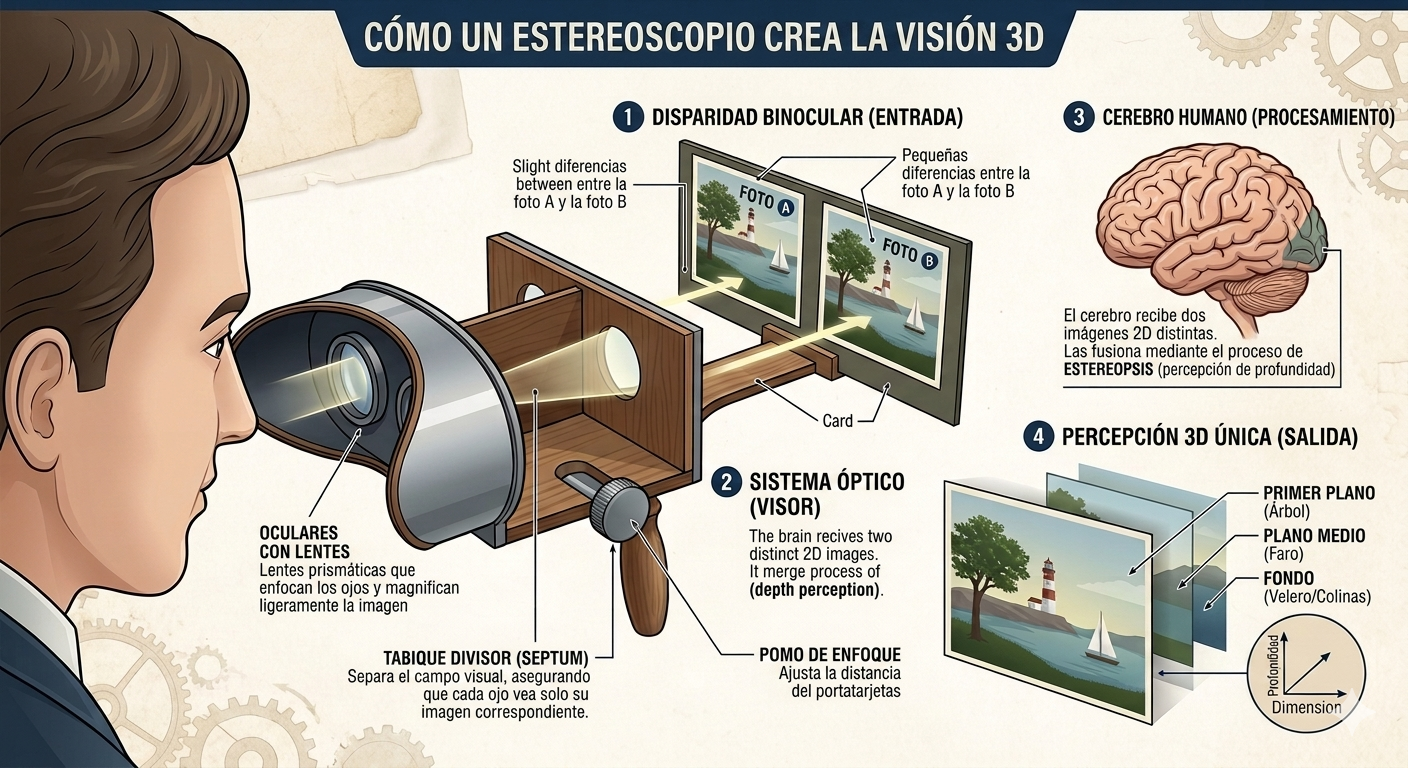
\includegraphics[width=0.85\linewidth]{00_Intro_VR/Stereoscope_ChatGPT.png}
\end{center}
\begin{center}
\tiny Image generated by AI assistant (ChatGpt) based on the prompt by Marco Aurelio Nuño-Maganda, May 28th, 2026.
\end{center}
\end{frame}




%
\begin{frame}{Realidad Virtual - Antecedente hist\'orico - estereoscopio}
Un estereoscopio (inventado alrededor del año 1851) proporciona im\'agenes separadas para cada ojo mediante lentes individuales, donde cada imagen tiene una variante en el angulo de captura y un desplazamiento horizontal.
\begin{center}
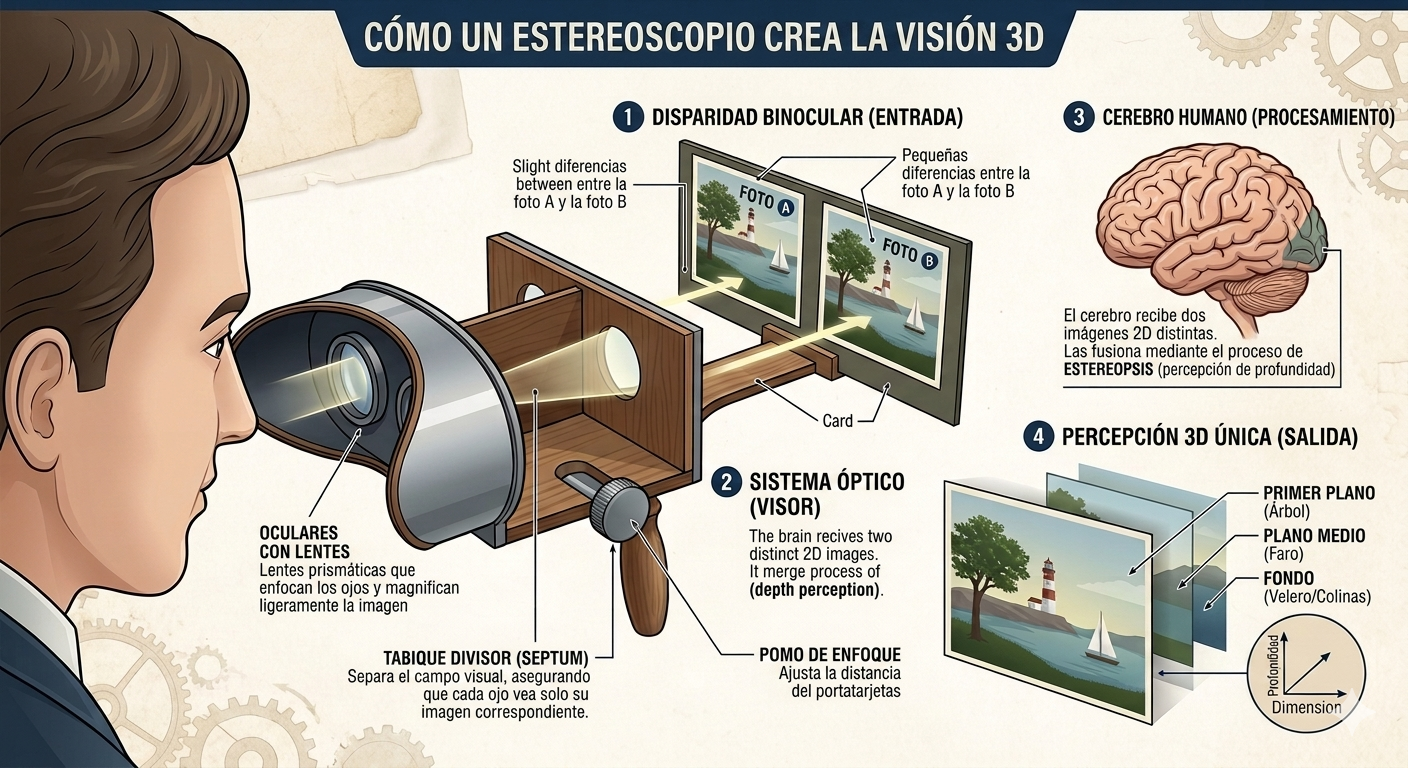
\includegraphics[width=0.75\linewidth]{00_Intro_VR/Stereoscope_ChatGPT.png}
\end{center}
\begin{center}
\tiny Image generated by AI assistant (ChatGpt) based on the prompt by Marco Aurelio Nuño-Maganda, May 28th, 2026.
\end{center}
\end{frame}


\begin{frame}{Realidad Virtual - Antecedente hist\'orico - View-Master}

\begin{itemize}
\item El View-Master funciona exactamente bajo el mismo principio óptico que un estereoscopio tradicional, pero compactado en un formato de juguete mecánico portátil.
\item El corazón del juguete es un disco de cartón, que contiene 7 pares de diapositivas transparentes a color dispuestas en círculos concéntricos
\end{itemize}



\begin{columns}
\begin{column}{0.49\textwidth}
\begin{center}
	\begin{tabular}{cc}
        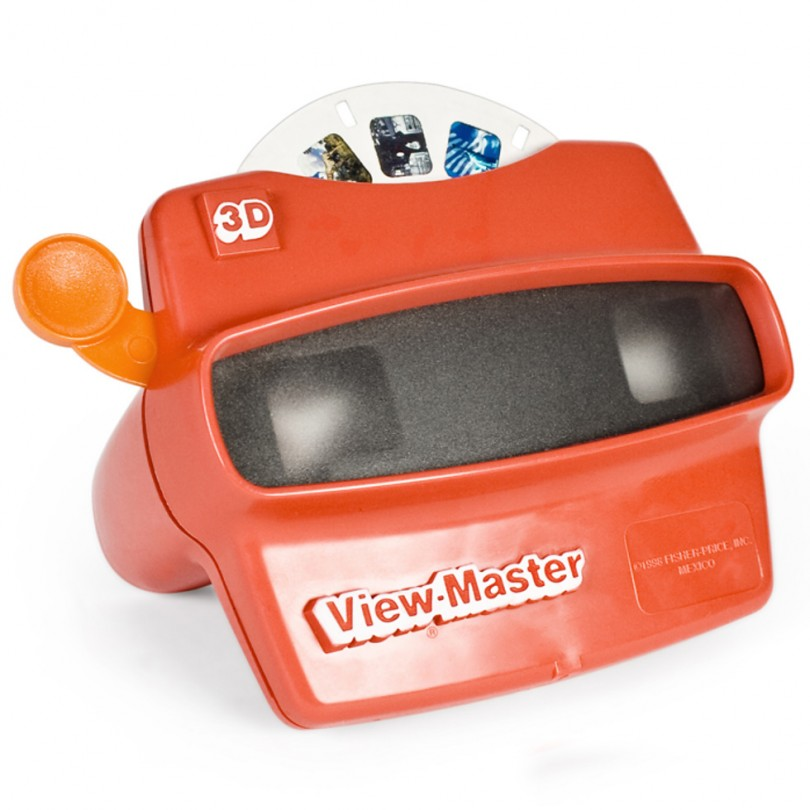
\includegraphics[width=0.49\linewidth]{Figs/view_master_blog-810x810.jpg} &
		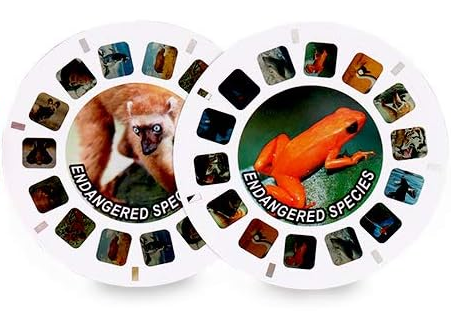
\includegraphics[width=0.49\linewidth]{Figs/DiscosViewMaster.png}    
	\end{tabular}
\end{center}
\end{column}

\begin{column}{0.49\textwidth}
    \begin{center}
        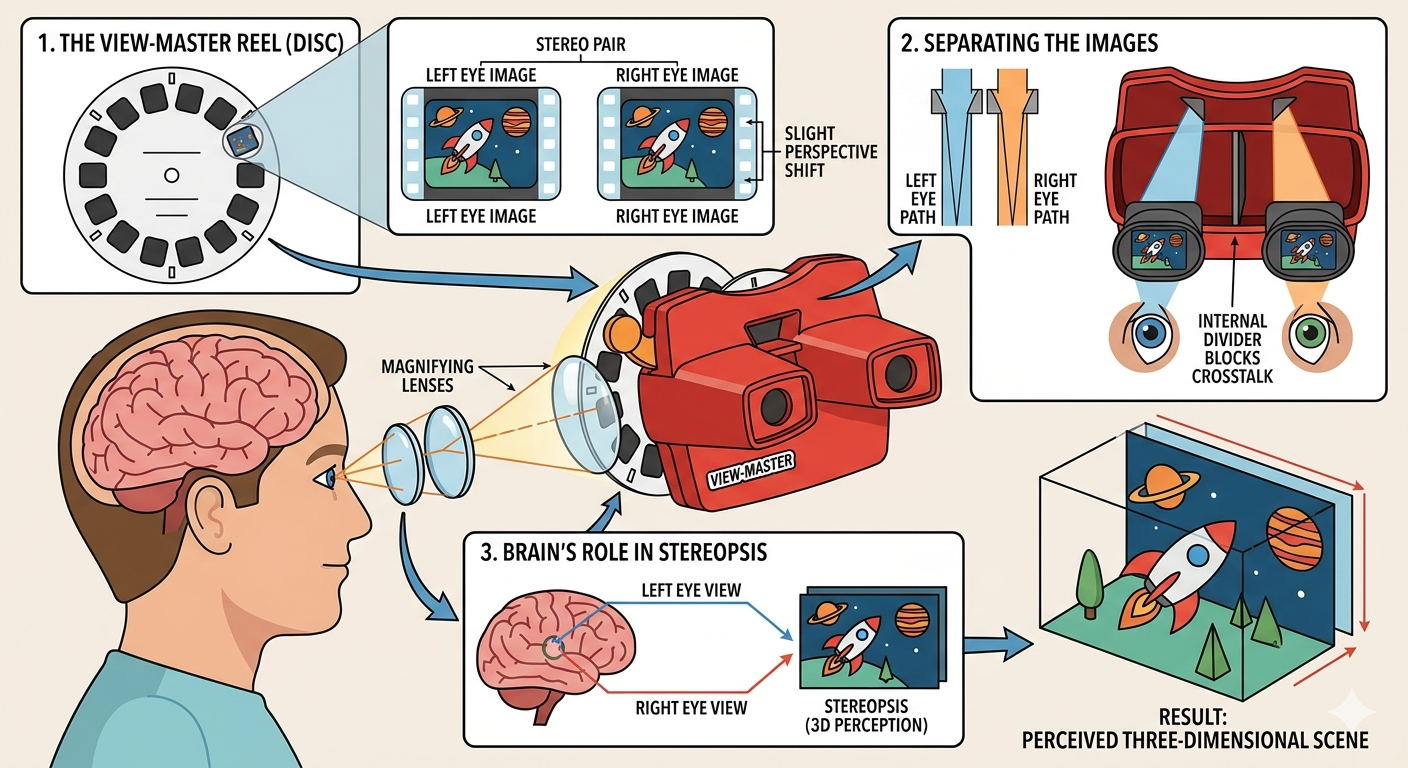
\includegraphics[width=0.99\linewidth]{00_Intro_VR/ViewMaster_ChatGPT.png}
    \end{center}
    \begin{center}
        \tiny Image generated by AI assistant (Gemini AI) based on the prompt by Marco Aurelio Nuño-Maganda, May 28th, 2026.
    \end{center}
\end{column}

\end{columns}
	
\end{frame}




\begin{frame}{Realidad Virtual (VR)}
%\begin{block}{Realidad Virtual (VR)} 
		\begin{itemize}
			\item La Realidad virtual (RV) emplea modelos y simulaciones por computadora que permite a una persona interactuar con un entorno visual artificial tridimensional (3D)
			\item En un formato típico de RV, un usuario lleva un casco con una pantalla estereoscópica para ver imágenes animadas de un entorno simulado
			\item El dispositivo m\'as econ\'omico para aplicaciones de RV es un tel\'efono inteligente 
		\end{itemize}
    \begin{center}
	\begin{tabular}{ccc}
    	\centering
		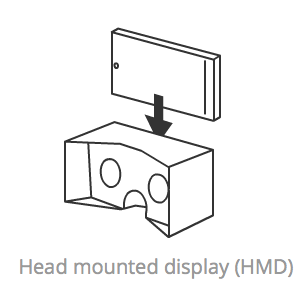
\includegraphics[width=0.25\linewidth]{Figs/MobileVR2} & 
        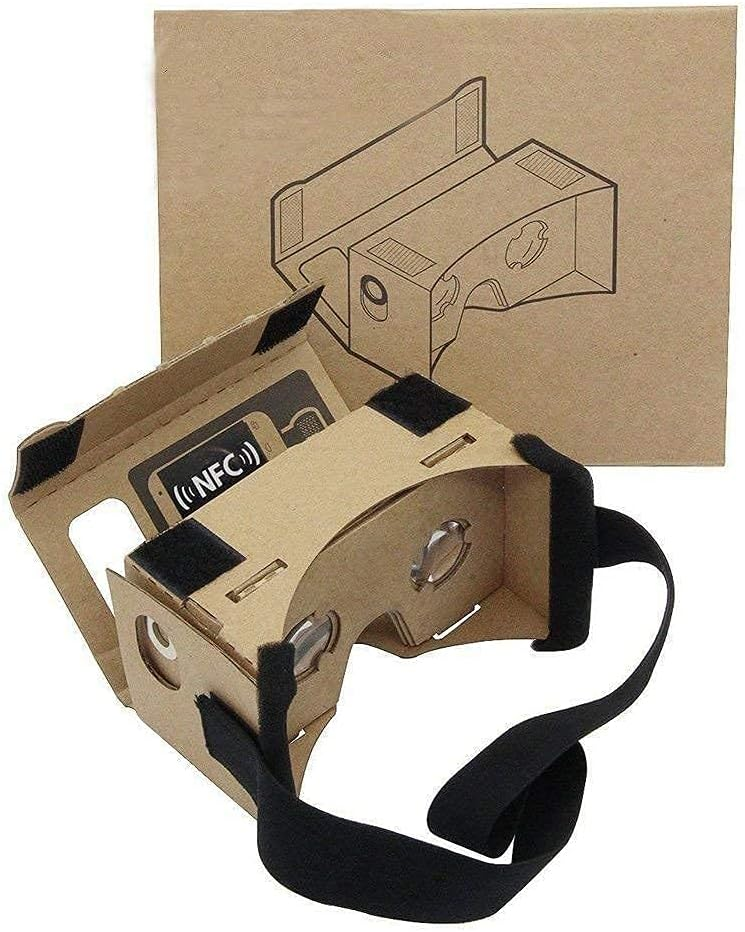
\includegraphics[width=0.19\linewidth]{Figs/CardBoard} & 		
        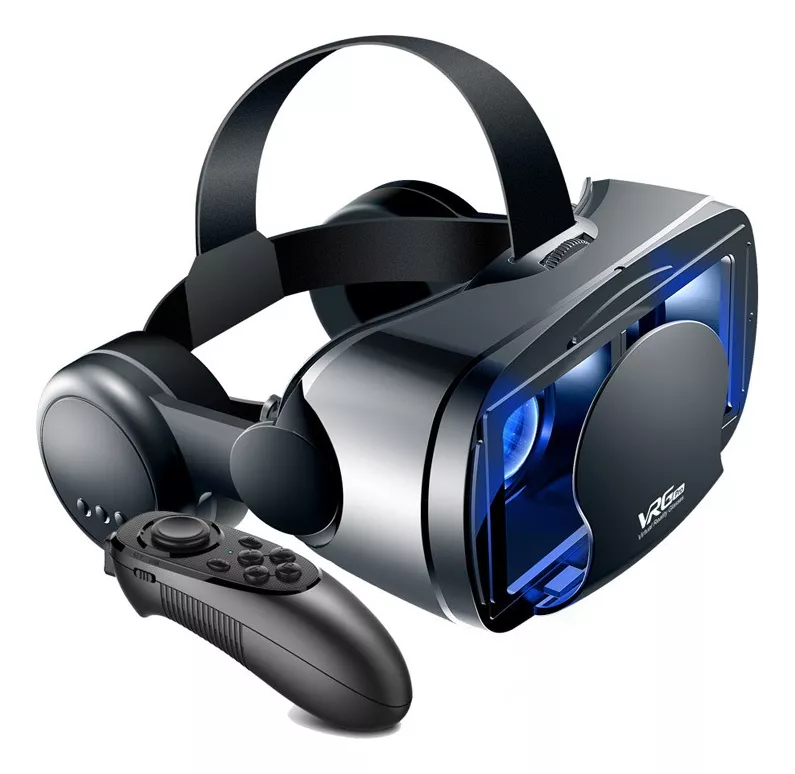
\includegraphics[width=0.19\linewidth]{Figs/VRGPro} 		
	\end{tabular}
		 \end{center}
%\end{block} 
\footnotetext{\url{https://reference.codeproject.com/book/dom/webvr_api/webvr_concepts}}
\end{frame}


\begin{frame}{Costos de Dispostivos HeadSets para VR}
\begin{columns}
\begin{column}{0.49\textwidth}
\begin{itemize}
\item Meta Quest 3 (499 USD)
\item Sony PlayStation VR2 (599 USD)
\item Meta Quest Pro (900 USD)
\item Valve Index VR Kit (1350 USD)
\item HTC Vive Pro 2 (1400 USD)
\end{itemize}

\begin{center}
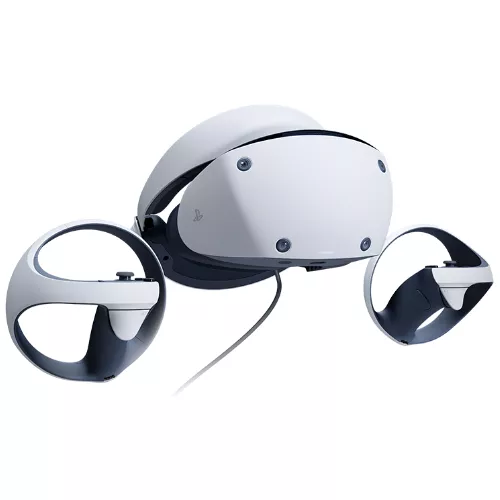
\includegraphics[width=0.75\textwidth]{Figs/sony.png}
\end{center}
\end{column}
\begin{column}{0.49\textwidth}
\begin{center}
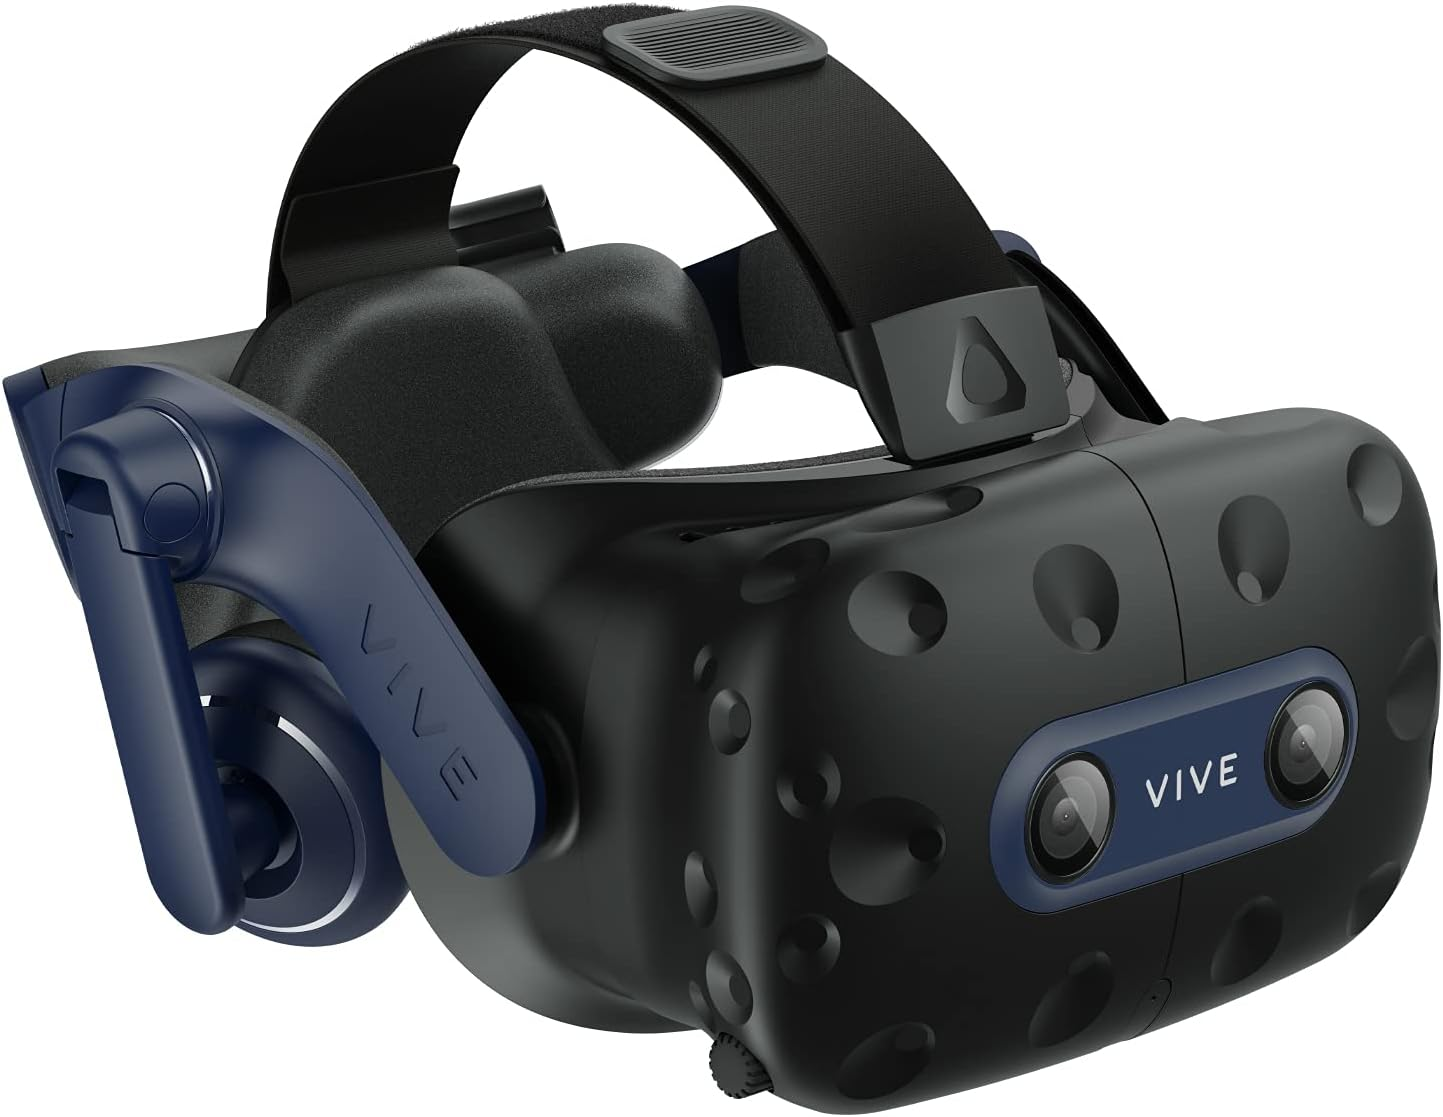
\includegraphics[width=0.75\textwidth]{Figs/HTC.jpg}\\
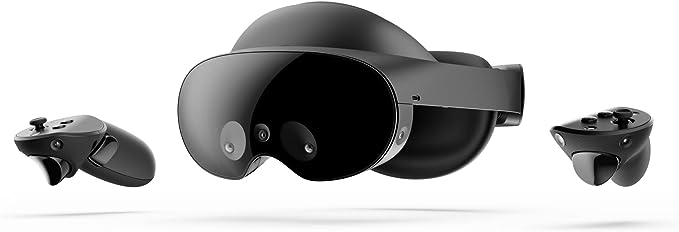
\includegraphics[width=0.95\textwidth]{Figs/MetaPro.jpg}
\end{center}
\end{column}
\end{columns}
\end{frame}


\begin{frame}{Relación entre RV - Teléfonos Inteligentes}
Los teléfonos inteligentes son una de las principales plataformas para sistemas de realidad virtual (VR):  
\begin{itemize}
\item Tienen hardware avanzado (cámaras, sensores de movimiento, procesadores gráficos) que permiten ejecutar experiencias inmersivas de VR sin necesidad de equipos especializados.  
\item Existen accesorios como \textbf{gafas VR para móviles} (ej. Google Cardboard, Samsung Gear VR) que convierten un teléfono en un visor de realidad virtual.  
\item Existen herramientas para crear apps de  RV
\item Muchas aplicaciones combinan AR con inteligencia artificial para ofrecer experiencias interactivas y personalizadas.  
\item Gran cantidad de aplicaciones prácticas
\end{itemize}
\end{frame}


\begin{frame}{Realidad Virtual - Antecedente hist\'orico}

\begin{columns}
\begin{column}{0.49\textwidth}


\begin{itemize}
\item Un estereoscopio proporciona im\'agenes separadas para cada ojo mediante lentes individuales, donde cada imagen tiene una variante en el angulo de captura y un desplazamiento horizontal.
\item El cerebro de una persona con una percepción binocular normal de la profundidad al utilizar el estereoscopio ``mezcla'' ambas imagenes para crear una  ``ventana estereoscópica''
\end{itemize}
\end{column}

\begin{column}{0.49\textwidth}

\begin{center}
	\begin{tabular}{cc}
        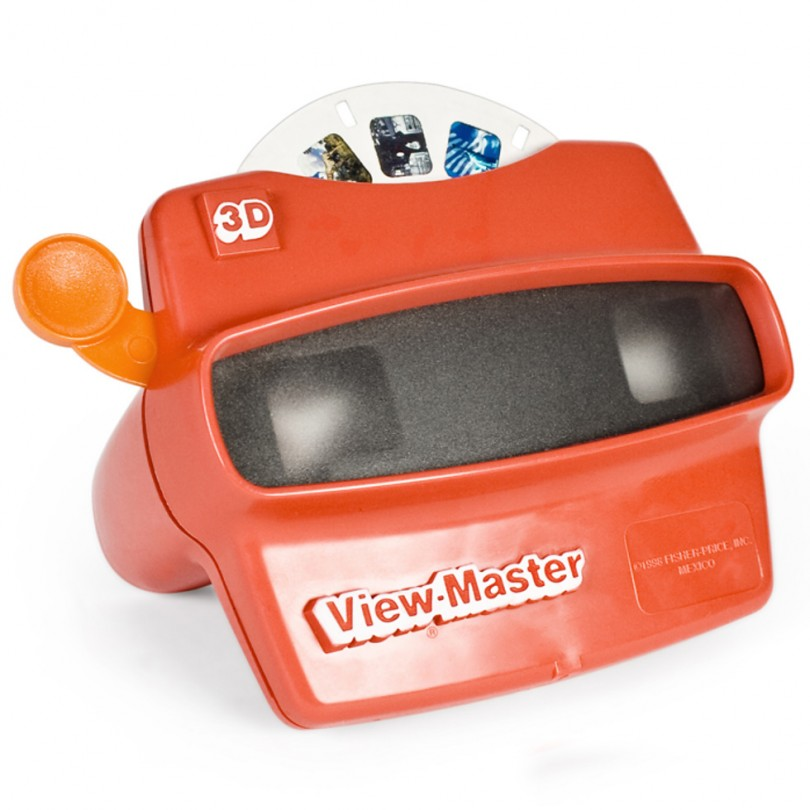
\includegraphics[width=0.45\linewidth]{Figs/view_master_blog-810x810.jpg} &
		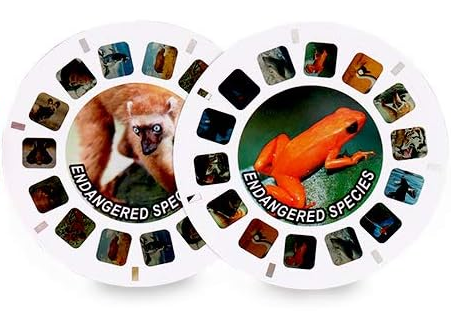
\includegraphics[width=0.45\linewidth]{Figs/DiscosViewMaster.png}    
	\end{tabular}

	\begin{tabular}{cc}
	\centering
        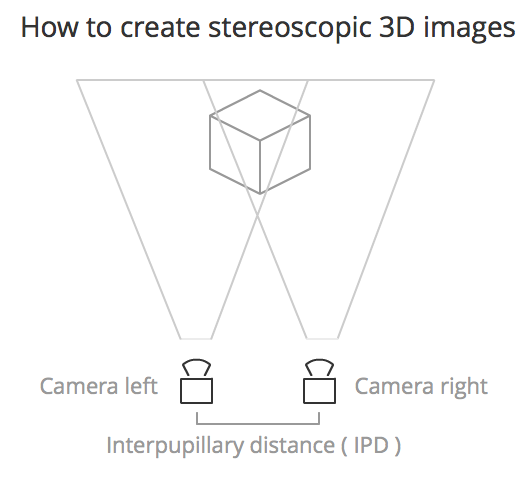
\includegraphics[width=0.49\linewidth]{Figs/VirtualReal1} &
        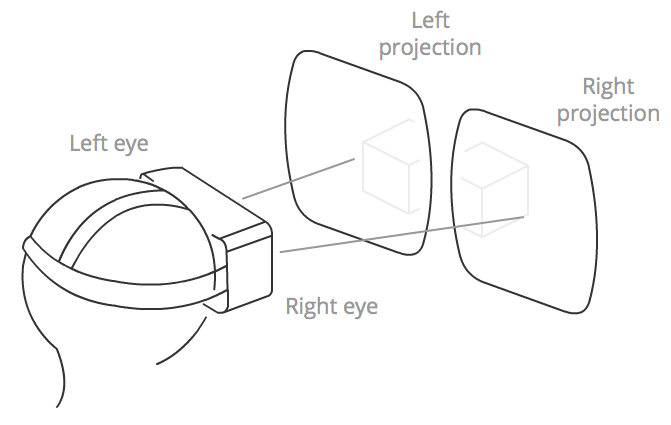
\includegraphics[width=0.49\linewidth]{Figs/VirtualReal2} \\

	\end{tabular}
\end{center}
\end{column}

\end{columns}

\end{frame}




\begin{frame}{Realidad Virtual (VR)}
%\begin{block}{Realidad Virtual (VR)} 
		\begin{itemize}
			\item La Realidad virtual (RV) emplea modelos y simulaciones por computadora que permite a una persona interactuar con un entorno visual artificial tridimensional (3D)
			\item En un formato típico de RV, un usuario lleva un casco con una pantalla estereoscópica para ver imágenes animadas de un entorno simulado
			\item El dispositivo m\'as econ\'omico para aplicaciones de RV es un tel\'efono inteligente 
		\end{itemize}
    \begin{center}
	\begin{tabular}{ccc}
    	\centering
		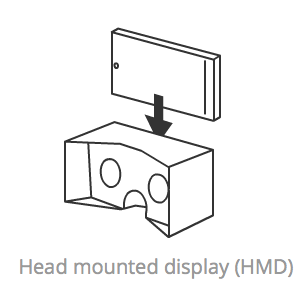
\includegraphics[width=0.25\linewidth]{Figs/MobileVR2} & 
        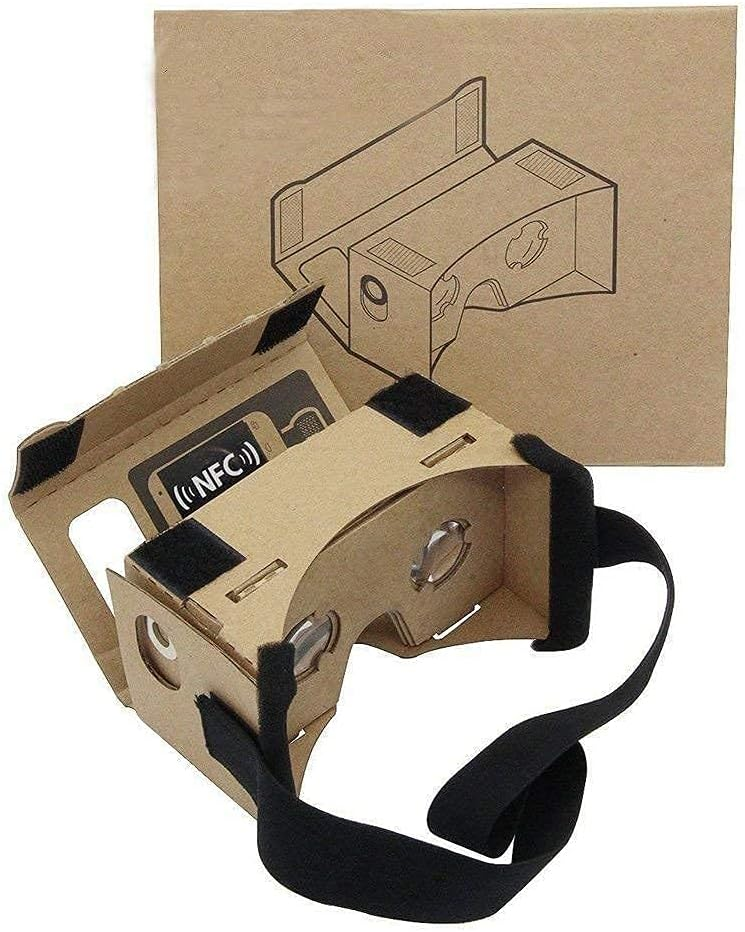
\includegraphics[width=0.19\linewidth]{Figs/CardBoard} & 		
        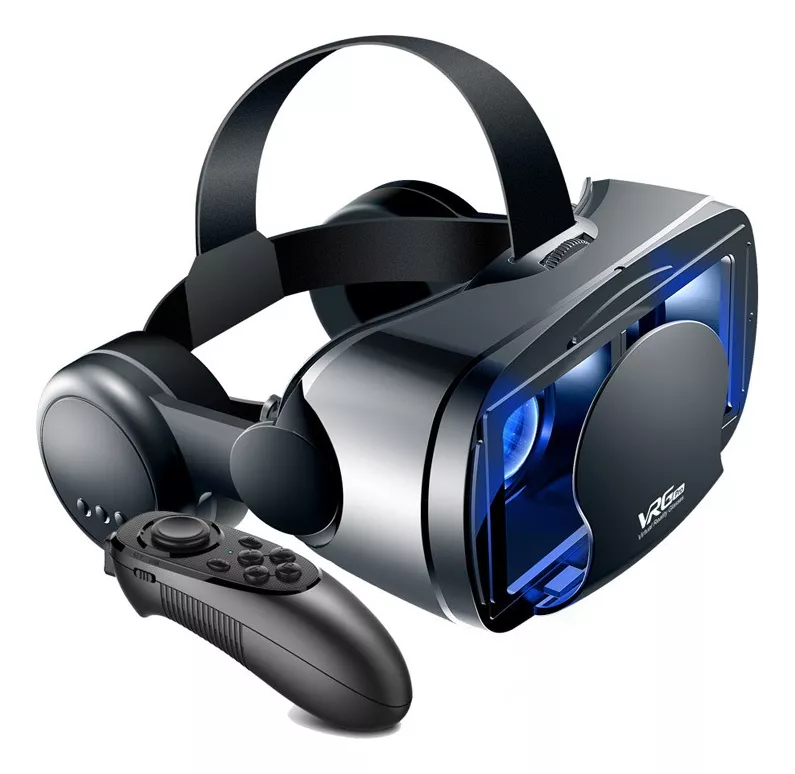
\includegraphics[width=0.19\linewidth]{Figs/VRGPro} 		
	\end{tabular}
		 \end{center}
%\end{block} 
\footnotetext{\url{https://reference.codeproject.com/book/dom/webvr_api/webvr_concepts}}
\end{frame}





\section[PRV]{Recorridos Virtuales}


\begin{frame}{Recorridos Virtuales y Uso de Teléfonos Inteligentes}

\textbf{¿Qué son los recorridos virtuales?}
\begin{itemize}
    \item Son representaciones digitales interactivas de espacios reales o simulados.
    \item Se utilizan en turismo, educación, bienes raíces y museos.
\end{itemize}
\vspace{0.5cm}
\begin{center}
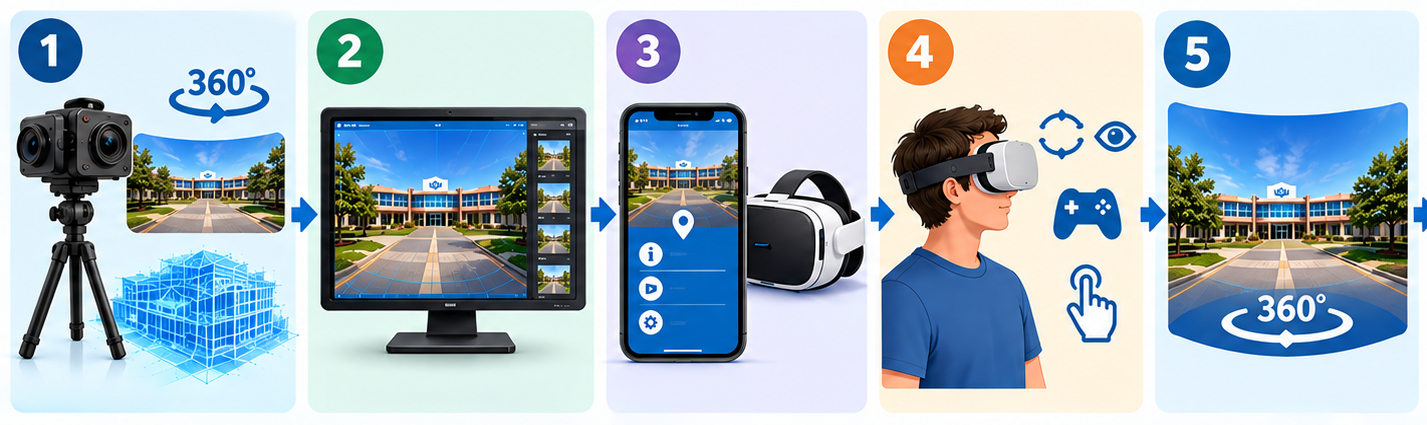
\includegraphics[width=0.85\linewidth]{00_IntroRecorridosVirtuales/Flujo_de_un_recorrido_virtual_en_RV.png}
\end{center}
 \begin{center}
        \tiny Image generated by AI assistant (ChatGPT) based on the prompt by Marco Aurelio Nuño-Maganda, Oct 14th, 2026.
    \end{center}


\end{frame}



\begin{frame}{Recorridos Virtuales Desarrollados en la UPV}

Principalmente desarrollados con ayuda de estudiantes de la carrera de \textbf{Ingeniería en Tecnologías de la Información (ITI)/Ingeniería en Tecnologías de la Información e Innovación Digital (ITIID)} de la \textit{Universidad Politécnica de Victoria}.

Materiales:
\begin{itemize}
\item Un teléfono inteligente con Android y soporte para realidad virtual.
\item Un control de XBox (o Genérico) vinculado con el telefono inteligente (Bluetooth). 
\item Una carcasa para realidad virtual. 
\end{itemize}
Demos disponibles:
\begin{itemize}
\item Recorrido Virtual de la UPV.
\item Museo de Historia Regional de Tamaulipas.
\item Pinacoteca, Ciudad Victoria, Tamaulipas.
\item Casa del Arte, Ciudad Victoria, Tamaulipas.
\item Museo Tamux, Ciudad Victoria, Tamaulipas.
\end{itemize}
\end{frame}


%
\begin{frame}{Recorrido UPV Virtual en teléfonos inteligentes}
%\begin{block}{Recorrido UPV Virtual en teléfonos inteligentes} 
Demo incremental, que emplea OpenGL ES 2.0 (compatible con el 100\% de los smartphones). 
\begin{itemize}
\item Versión 1: Solo mundo virtual (no inmersivo). El usuario se movía con presionando teclas de la interfaz de usuario
\item Versión 2: Mundo virtual inmersivo (integrado a unos lentes). El usuario movía la vista mediante los datos obtenidos por el sensor giroscopio del teléfono inteligente y avanzaba usando un manos libres alámbrico.
\item Versión 3: Controlado por voz. El usuario se movía dentro del entorno mediante comandos de voz.
\item Versión 3.5: Controlado mediante control de videojuegos (Bluetooth o USB)
\end{itemize}
%\end{block} 
\end{frame}

\renewcommand{\EntradaBibtex}{Reporte2019}
\begin{frame}{\citetitle{\EntradaBibtex} \footnotemark[1] (1)}

%\begin{frame}{Recorrido UPV Virtual 1.0\footnotemark }
%\begin{block}{} 
\begin{columns}
\begin{column}{0.48\textwidth}
    \begin{center}

\begin{itemize}
\item La navegación es mediante botones (adelante, atrás, izquierda, derecha, subir, bajar)
\item Una potencial mejora es mediante eventos de toque en pantalla
\end{itemize}
     \end{center}

\end{column}
\begin{column}{0.52\textwidth}  
    \begin{center}
\begin{itemize}
\end{itemize}
     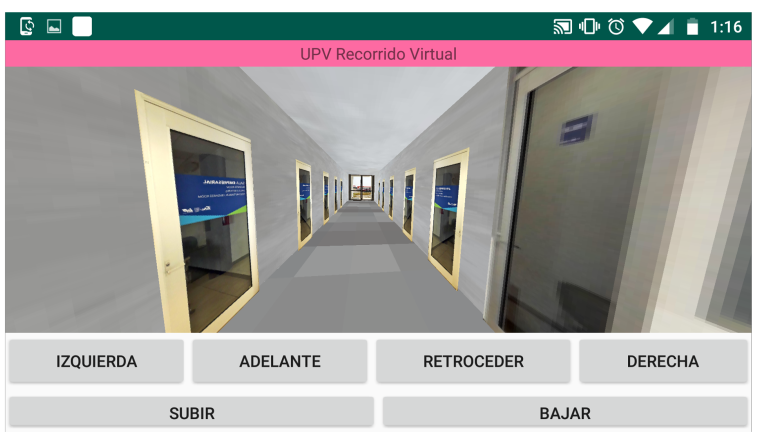
\includegraphics[width=0.9\textwidth]{Figs/RecorridoUPV_V1}\\
     \end{center}
\end{column}
\end{columns}
%\end{block} 
\footnotetext[1]{\fullcite{\EntradaBibtex}}
%\footnotetext{Baez Zapata Marıa Fernanda, Cárdenas Castillo Jesús Alfredo, Olvera Osuna José Armando and Wang Yu Hsiang. \textbf{Recorrido UPV en Android}. Proyecto Final de la Asignatura ``Cómputo en Dispositivos Móviles'', 2019. Sin Publicar.}
%\\setcounter{footnote}{0}
\end{frame}


%\begin{frame}{Recorrido UPV Virtual 1.0 (2)}
%\renewcommand{\EntradaBibtex}{Reporte2019}
\begin{frame}{\citetitle{\EntradaBibtex}  (2)}
%\begin{block}{Recorrido UPV Virtual 1.0 (2)} 
\begin{itemize}
\item Vistas de los diferentes edificios
\end{itemize}
    \begin{center}
     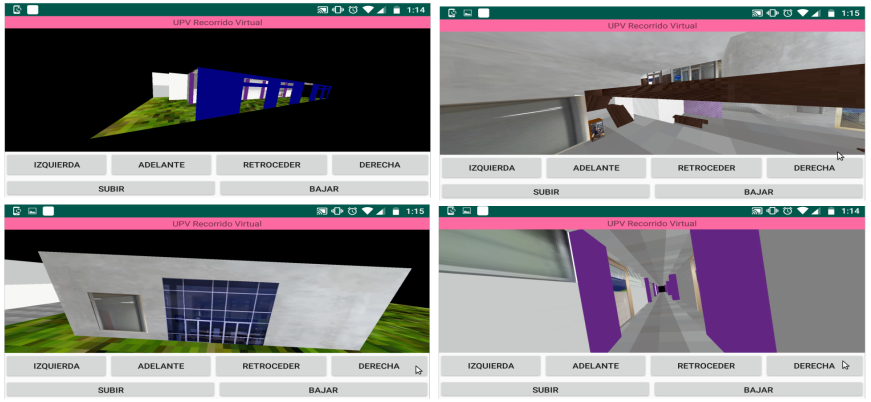
\includegraphics[width=0.80\textwidth]{Figs/RecorridoUPV_V2}\\
     \end{center}
%\end{block} 
\end{frame}

\renewcommand{\EntradaBibtex}{RecorridoVirtualLentesVR_2019}
%\begin{frame}{Recorrido UPV Virtual 2.0\footnotemark}
\begin{frame}{\citetitle{\EntradaBibtex}  (2)}
%\begin{block}{Recorrido UPV Virtual 2.0\footnotemark} 
\begin{columns}
\begin{column}{0.48\textwidth}
    \begin{center}

\begin{itemize}
\item Se extendió el demo 1.0 para generar una vista dual, requerida para su uso en conjunto con un armazón de VR.
\item La vista cambia en base a lo obtenido por el giroscopio, y el movimiento se controla mediante el botón del manos libres.
\end{itemize}
     \end{center}

\end{column}
\begin{column}{0.52\textwidth}  
    \begin{center}
\begin{itemize}
\end{itemize}
     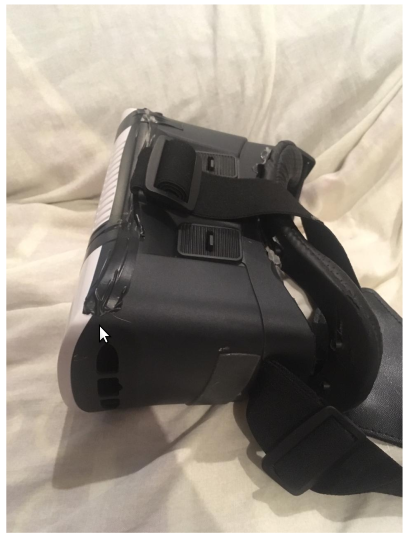
\includegraphics[width=0.4\textwidth]{Figs/RecorridoUPV_V3}\\
     \end{center}
\end{column}
\end{columns}
%\end{block} 
%\footnotetext{\fullcite{RecorridoVirtualLentesVR_2019}}
\footnotetext[1]{\fullcite{\EntradaBibtex}}
%\footnotetext{Alarcon Longoria Carlos Alberto, Alonso Cepeda Leonardo Daniel and Torres Grimaldo Luis Angel. \textbf{Recorrido UPV Virtual en Android}.  Proyecto Final de la Asignatura ``Cómputo en Dispositivos Móviles'', 2019. Sin Publicar.}
%\\setcounter{footnote}{0}
\end{frame}


\renewcommand{\EntradaBibtex}{RecorridoVirtualLentes_ComandosVoz2020}
\begin{frame}{\citetitle{\EntradaBibtex}  (1)}
%\begin{block}{Recorrido UPV Virtual 3.0\footnotemark} 
\begin{columns}
\begin{column}{0.48\textwidth}
    \begin{center}
\begin{itemize}
\item Se eliminó el uso del botón del manos libres para incluir comandos de voz
\item La aplicación respondía a los comandos de voz, de tal forma que el usuario no debería mover nada
\end{itemize}
     \end{center}

\end{column}
\begin{column}{0.52\textwidth}  
    \begin{center}
     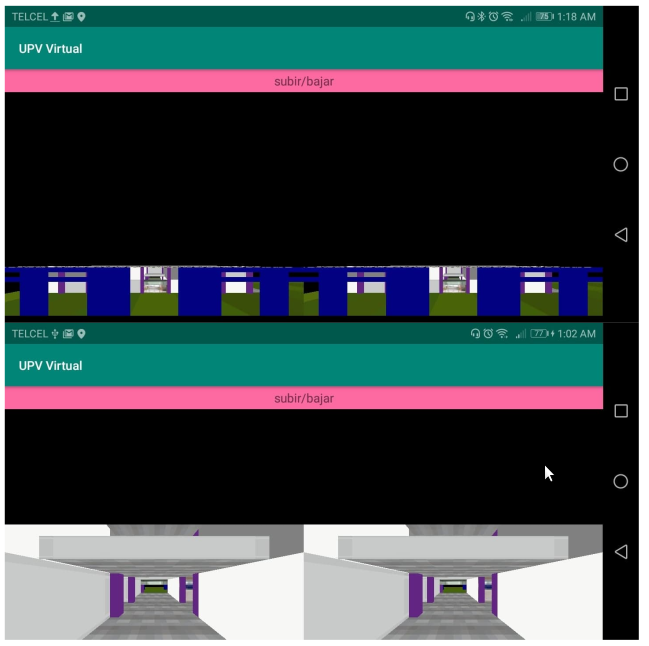
\includegraphics[width=0.6\textwidth]{Figs/RecorridoUPV_V5}\\
     \end{center}
\end{column}
\end{columns}
%\end{block} 
\footnotetext[1]{\fullcite{\EntradaBibtex}}
%\footnotetext{José Treviño Olvera. \textbf{Recorrido UPV Virtual en Android con Controles de Voz.}  Proyecto Final de la Asignatura. ``Cómputo en Dispositivos Móviles'', 2020. Sin Publicar.}
%\\setcounter{footnote}{0}
\end{frame}

\renewcommand{\EntradaBibtex}{RecoridoUPV_controles_2021}
%\begin{frame}{Recorrido UPV Virtual 3.5 \footnotemark}
%\begin{block}{Recorrido UPV Virtual 3.5 \footnotemark } 
\begin{frame}{\citetitle{\EntradaBibtex}  (1)}
\begin{itemize}
\item Se incorporaron varios controles de consolas de videojuego para la navegación.
\end{itemize}
\begin{columns}
\begin{column}{0.48\textwidth}
\begin{center}
	\begin{tabular}{ccc}
		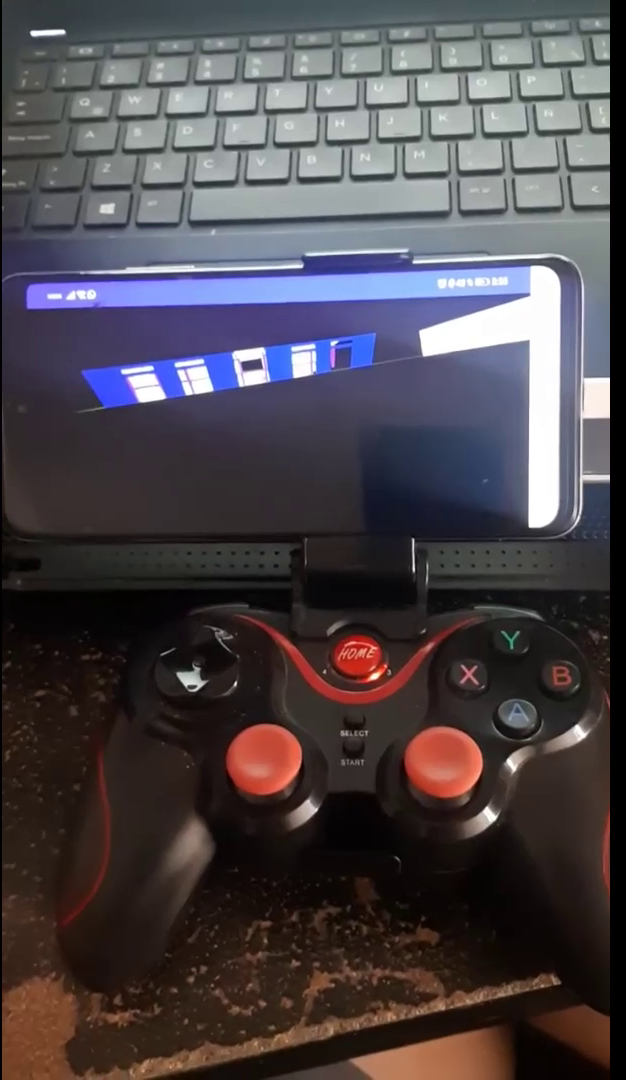
\includegraphics[width=0.25\linewidth]{Figs/UPV_Control01} & 		
		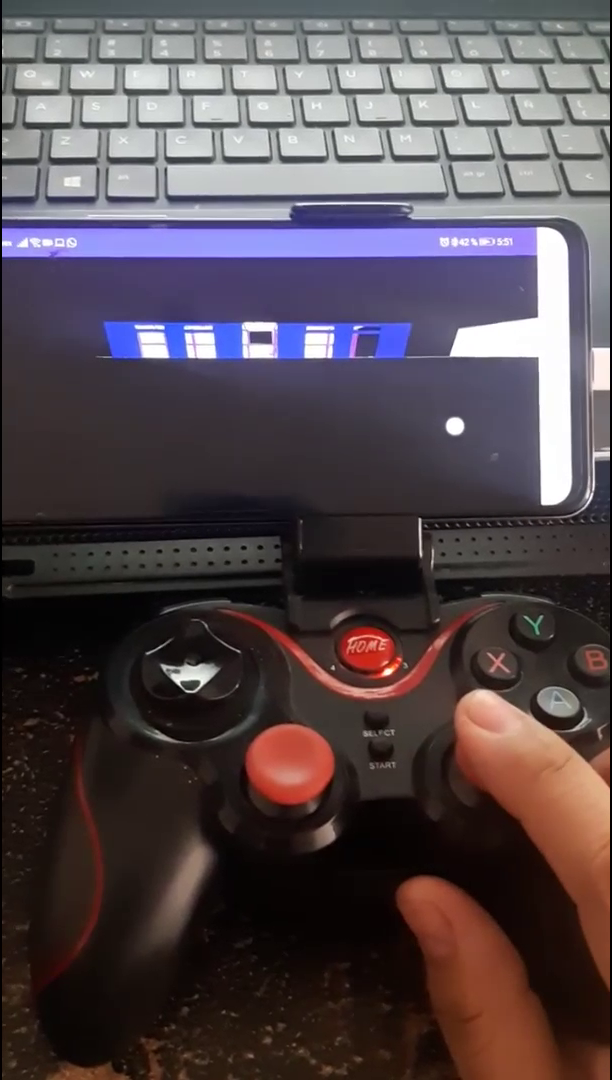
\includegraphics[width=0.25\linewidth]{Figs/UPV_Control02} & 
        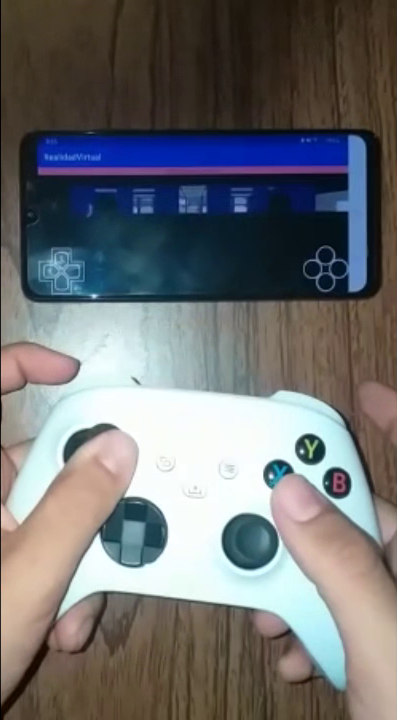
\includegraphics[width=0.25\linewidth]{Figs/UPV_Control04}\\
	\end{tabular}
\end{center}
\end{column}
\begin{column}{0.48\textwidth}
\begin{center}
	\begin{tabular}{c}
		    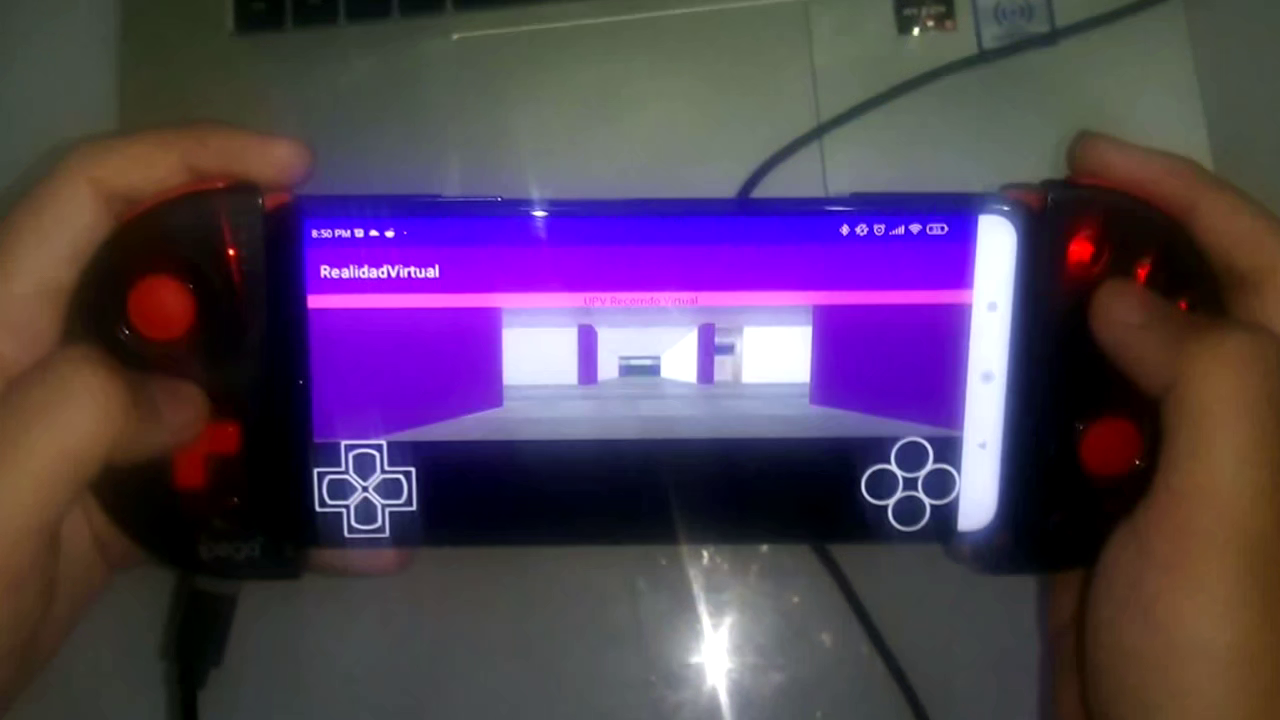
\includegraphics[width=0.45\linewidth]{Figs/UPV_Control03}\\
		    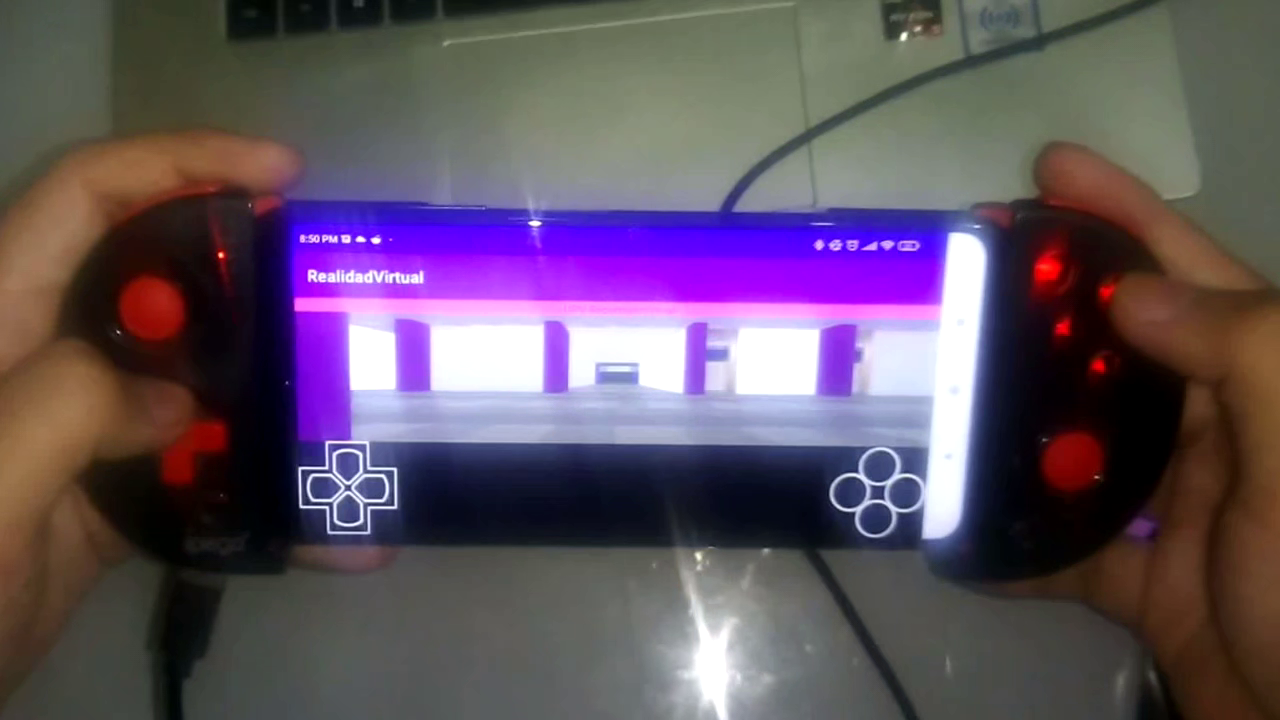
\includegraphics[width=0.45\linewidth]{Figs/UPV_Control05}\\
	\end{tabular}
\end{center}	
\end{column}
\end{columns}
%\end{block} 
\footnotetext[1]{\fullcite{\EntradaBibtex}}
%\footnotetext{\fullcite{RecoridoUPV_controles_2021}}
\end{frame}

 % Actualizacion

\renewcommand{\Folder}{2025_RecorridoUPV}
\renewcommand{\EntradaBibtex}{2025_RecorridoUPV}

\begin{frame}{\citetitle{\EntradaBibtex} \footnotemark[1] (1)}
\begin{columns}
	\begin{column}{0.48\textwidth}
		\begin{itemize}
			\item Se creo una aplicación móvil de Realidad Virtual que permite a los usuarios  mejorar su conocimiento sobre la ubicación de los estados en México. 
			\item Se muestra un lienzo con las piezas de los estados y un estado, el cual debe arrastrarse hasta colocarse en su posición correcta.
            \item El sistema valida si la pieza fue colocada en el lugar correcto y dar retroalimentación inmediata al usuario.
		\end{itemize}
	\end{column}
	\begin{column}{0.48\textwidth}
		\begin{center}
			\includegraphics[width=0.98\textwidth]{\Folder/figs/img1}
		\end{center}
		 \begin{center}
		     \includegraphics[width=0.98\textwidth]{\Folder/figs/img2}
		 \end{center}

	\end{column}
	
\end{columns}

%\end{block} 
\footnotetext[1]{\fullcite{\EntradaBibtex}}
\end{frame}


\begin{frame}{\citetitle{\EntradaBibtex}  (2)}
\begin{columns}
	\begin{column}{0.48\textwidth}
		\begin{itemize}
			\item Se creo una aplicación móvil de Realidad Virtual que permite a los usuarios  mejorar su conocimiento sobre la ubicación de los estados en México. 
			\item Se muestra un lienzo con las piezas de los estados y un estado, el cual debe arrastrarse hasta colocarse en su posición correcta.
            \item El sistema valida si la pieza fue colocada en el lugar correcto y dar retroalimentación inmediata al usuario.
		\end{itemize}
	\end{column}
	\begin{column}{0.48\textwidth}
		\begin{center}
			\includegraphics[width=0.98\textwidth]{\Folder/figs/img3}
		\end{center}
		 \begin{center}
		     \includegraphics[width=0.98\textwidth]{\Folder/figs/img4}
		 \end{center}

	\end{column}
	
\end{columns}

%\end{block} 
%\footnotetext[1]{\fullcite{\EntradaBibtex}}
\end{frame}

 % Actualizacion

\renewcommand{\EntradaBibtex}{MuseoRegionalVirtual_2023}

\begin{frame}{\citetitle{\EntradaBibtex}$^*$ (1)}
\begin{block}{Motivación} 
\begin{itemize}
\item Se implementó una aplicación móvil para explorar de manera interactiva el Museo Regional de Historia de Tamaulipas. 
\end{itemize}
\end{block} 
\begin{center}
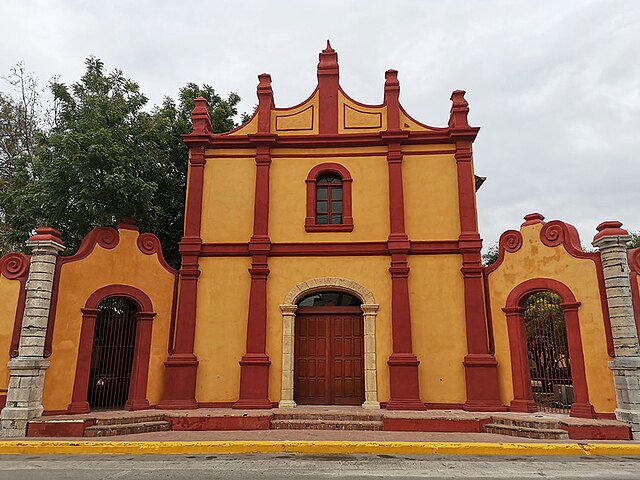
\includegraphics[width=0.38\linewidth]{2023_MuseoRegional_Virtual/Museo.jpg}
\end{center}
\footfullcite*{\EntradaBibtex}
\end{frame}


\begin{frame}{\citetitle{\EntradaBibtex} (2)}
%\begin{block}{Pantallas Principales} 

\begin{columns}
% Column 1
\column{.99\linewidth}



\begin{center}
	\begin{tabular}{cc}

		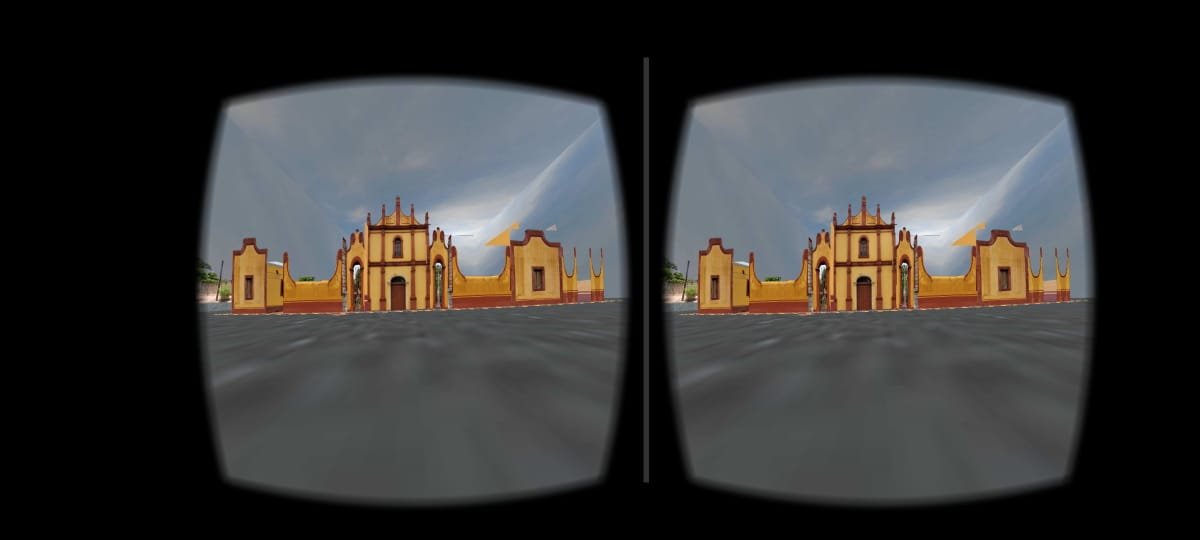
\includegraphics[width=0.45\linewidth]{2023_MuseoRegional_Virtual/1.jpeg} &
		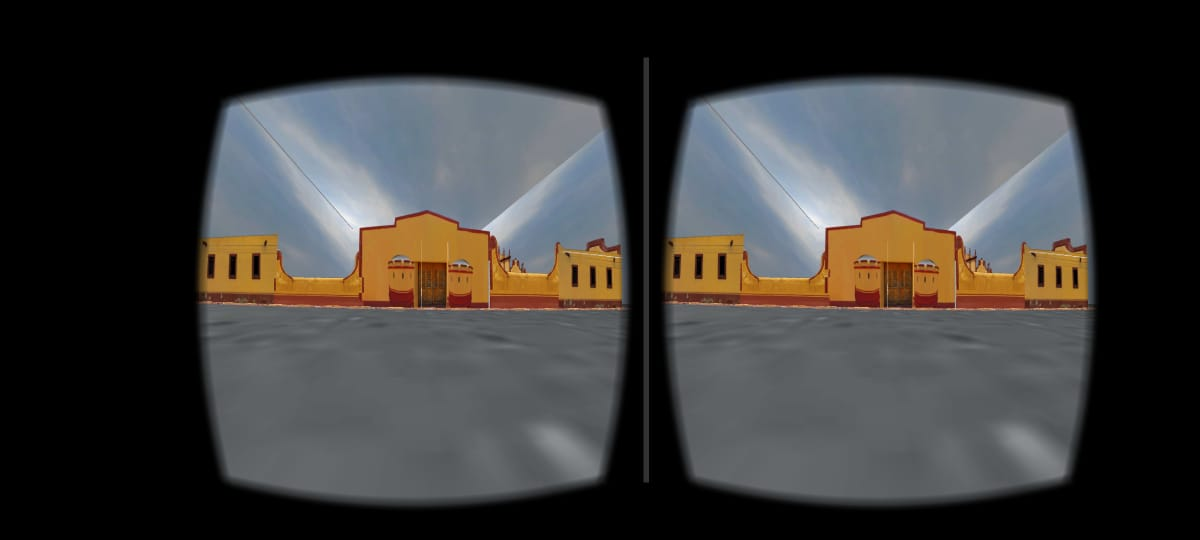
\includegraphics[width=0.45\linewidth]{2023_MuseoRegional_Virtual/2.jpeg} \\
		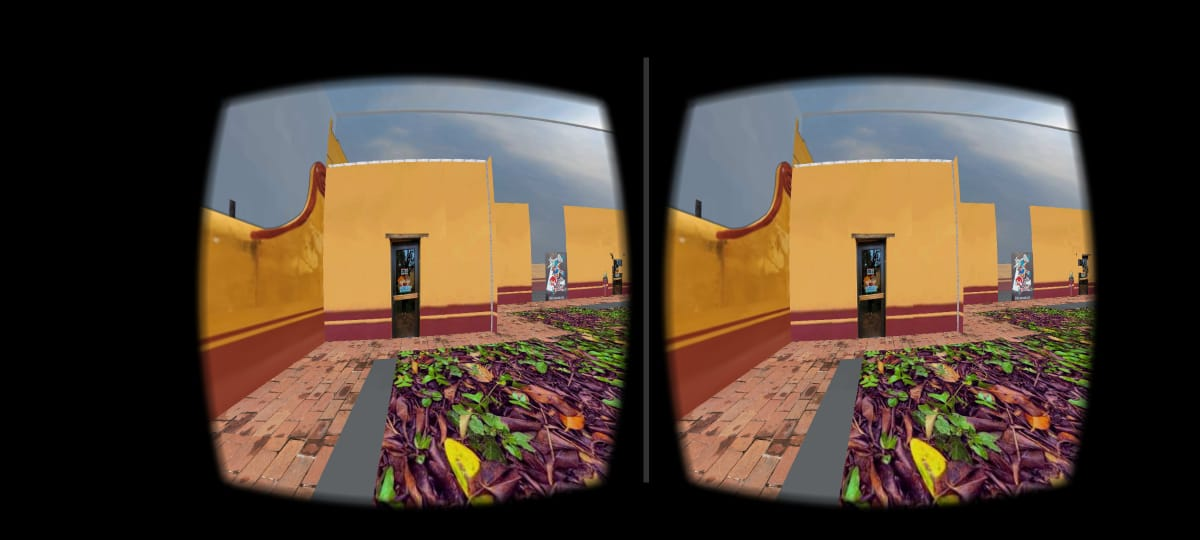
\includegraphics[width=0.45\linewidth]{2023_MuseoRegional_Virtual/6.jpeg} &
 		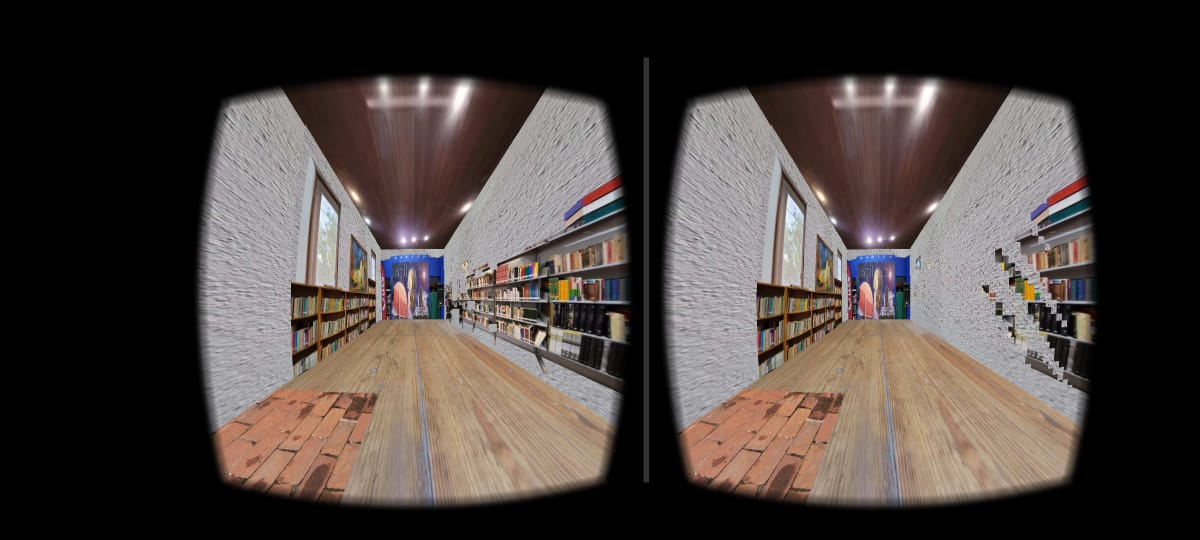
\includegraphics[width=0.45\linewidth]{2023_MuseoRegional_Virtual/7.jpeg} \\
	\end{tabular}
\end{center}



%\column{.5\linewidth}
%\begin{center}
	%\begin{tabular}{cccc}
	%	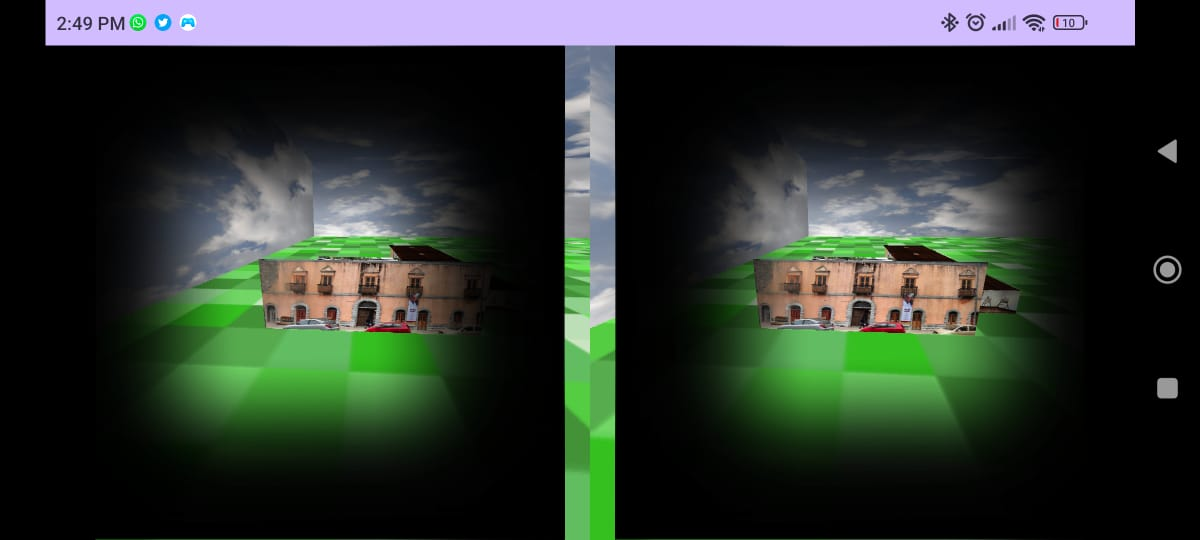
\includegraphics[width=0.40\linewidth]{2024_Pinacoteca_Virtual/PlanoGeneral.jpeg} &
 	%	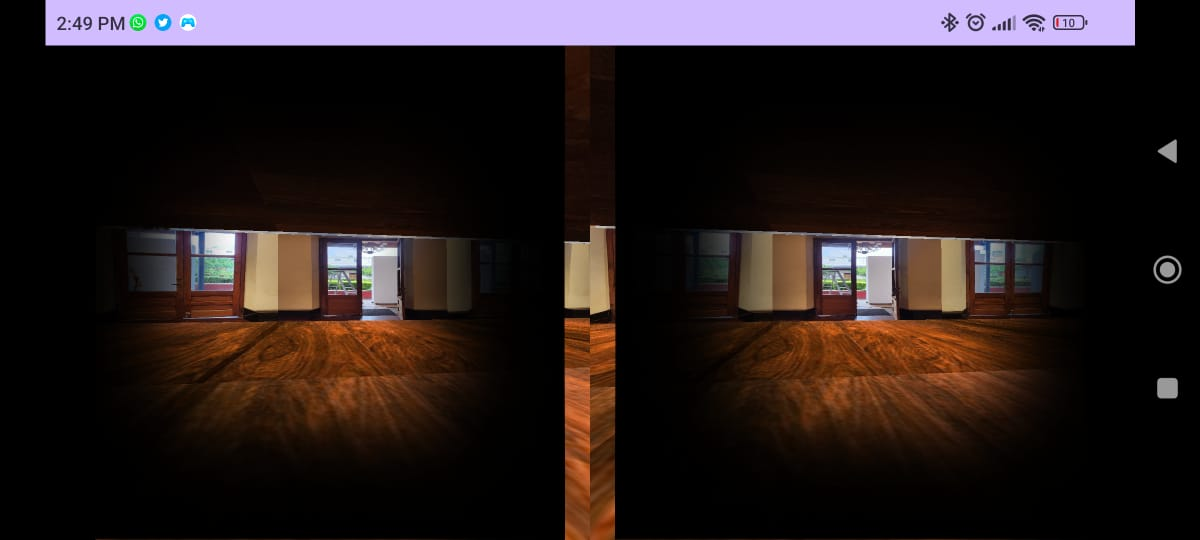
\includegraphics[width=0.40\linewidth]{2024_Pinacoteca_Virtual/Salida_SalonExhibiciones.jpeg} \\
%	\end{tabular}
%\end{center}


\end{columns}
\end{frame}




\renewcommand{\EntradaBibtex}{PinacotecaVirtual_2024}

\begin{frame}{\citetitle{\EntradaBibtex}$^*$ (1)}
\begin{block}{Motivación} 
\begin{itemize}
\item Se implementó una aplicación móvil para explorar de manera interactiva el museo virtual Pinacoteca de Tamaulipas. 
\end{itemize}
\end{block} 
\begin{center}
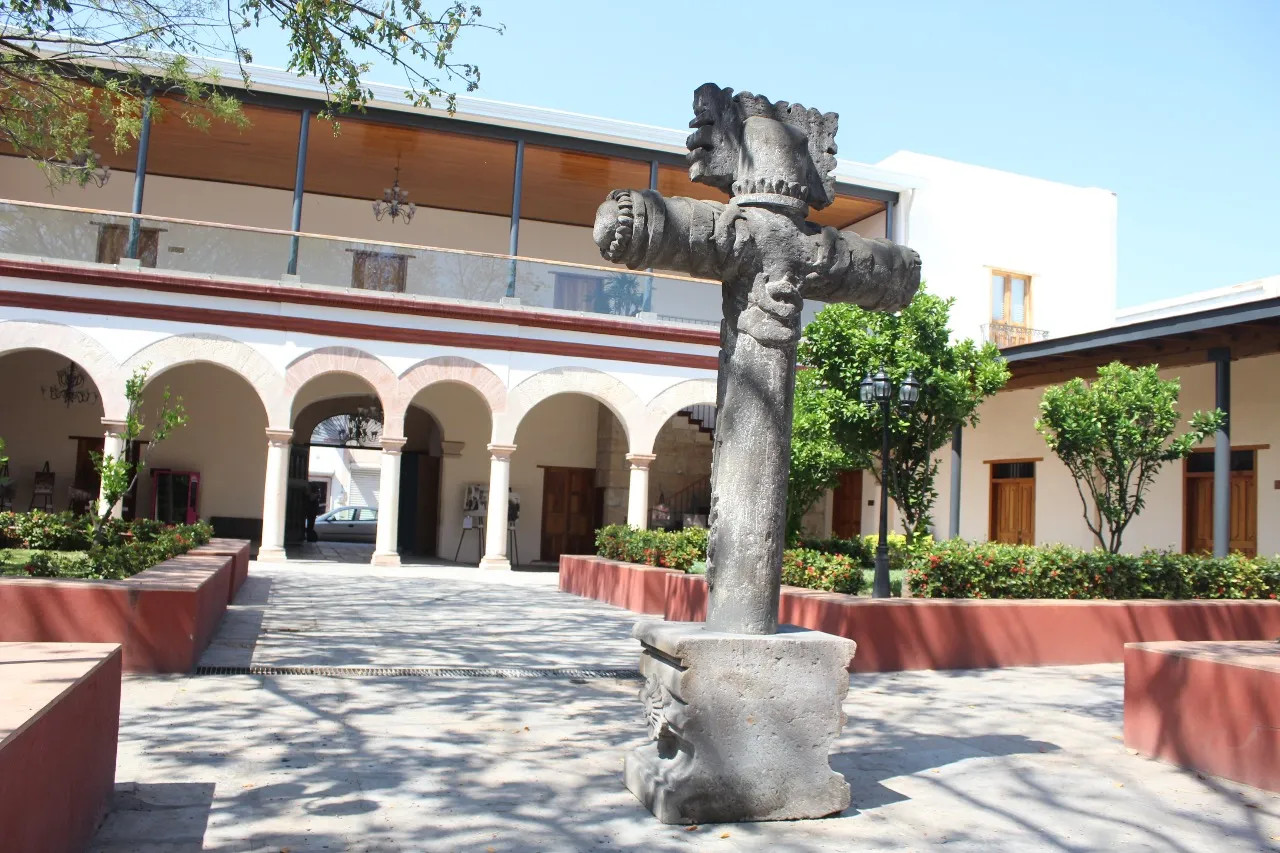
\includegraphics[width=0.38\linewidth]{2024_Pinacoteca_Virtual/casa-filizola2.jpg}
\end{center}
\footfullcite*{\EntradaBibtex}
\end{frame}


\begin{frame}{\citetitle{\EntradaBibtex} (2)}
%\begin{block}{Pantallas Principales} 

\begin{columns}
% Column 1
\column{.99\linewidth}



\begin{center}
	\begin{tabular}{cc}
		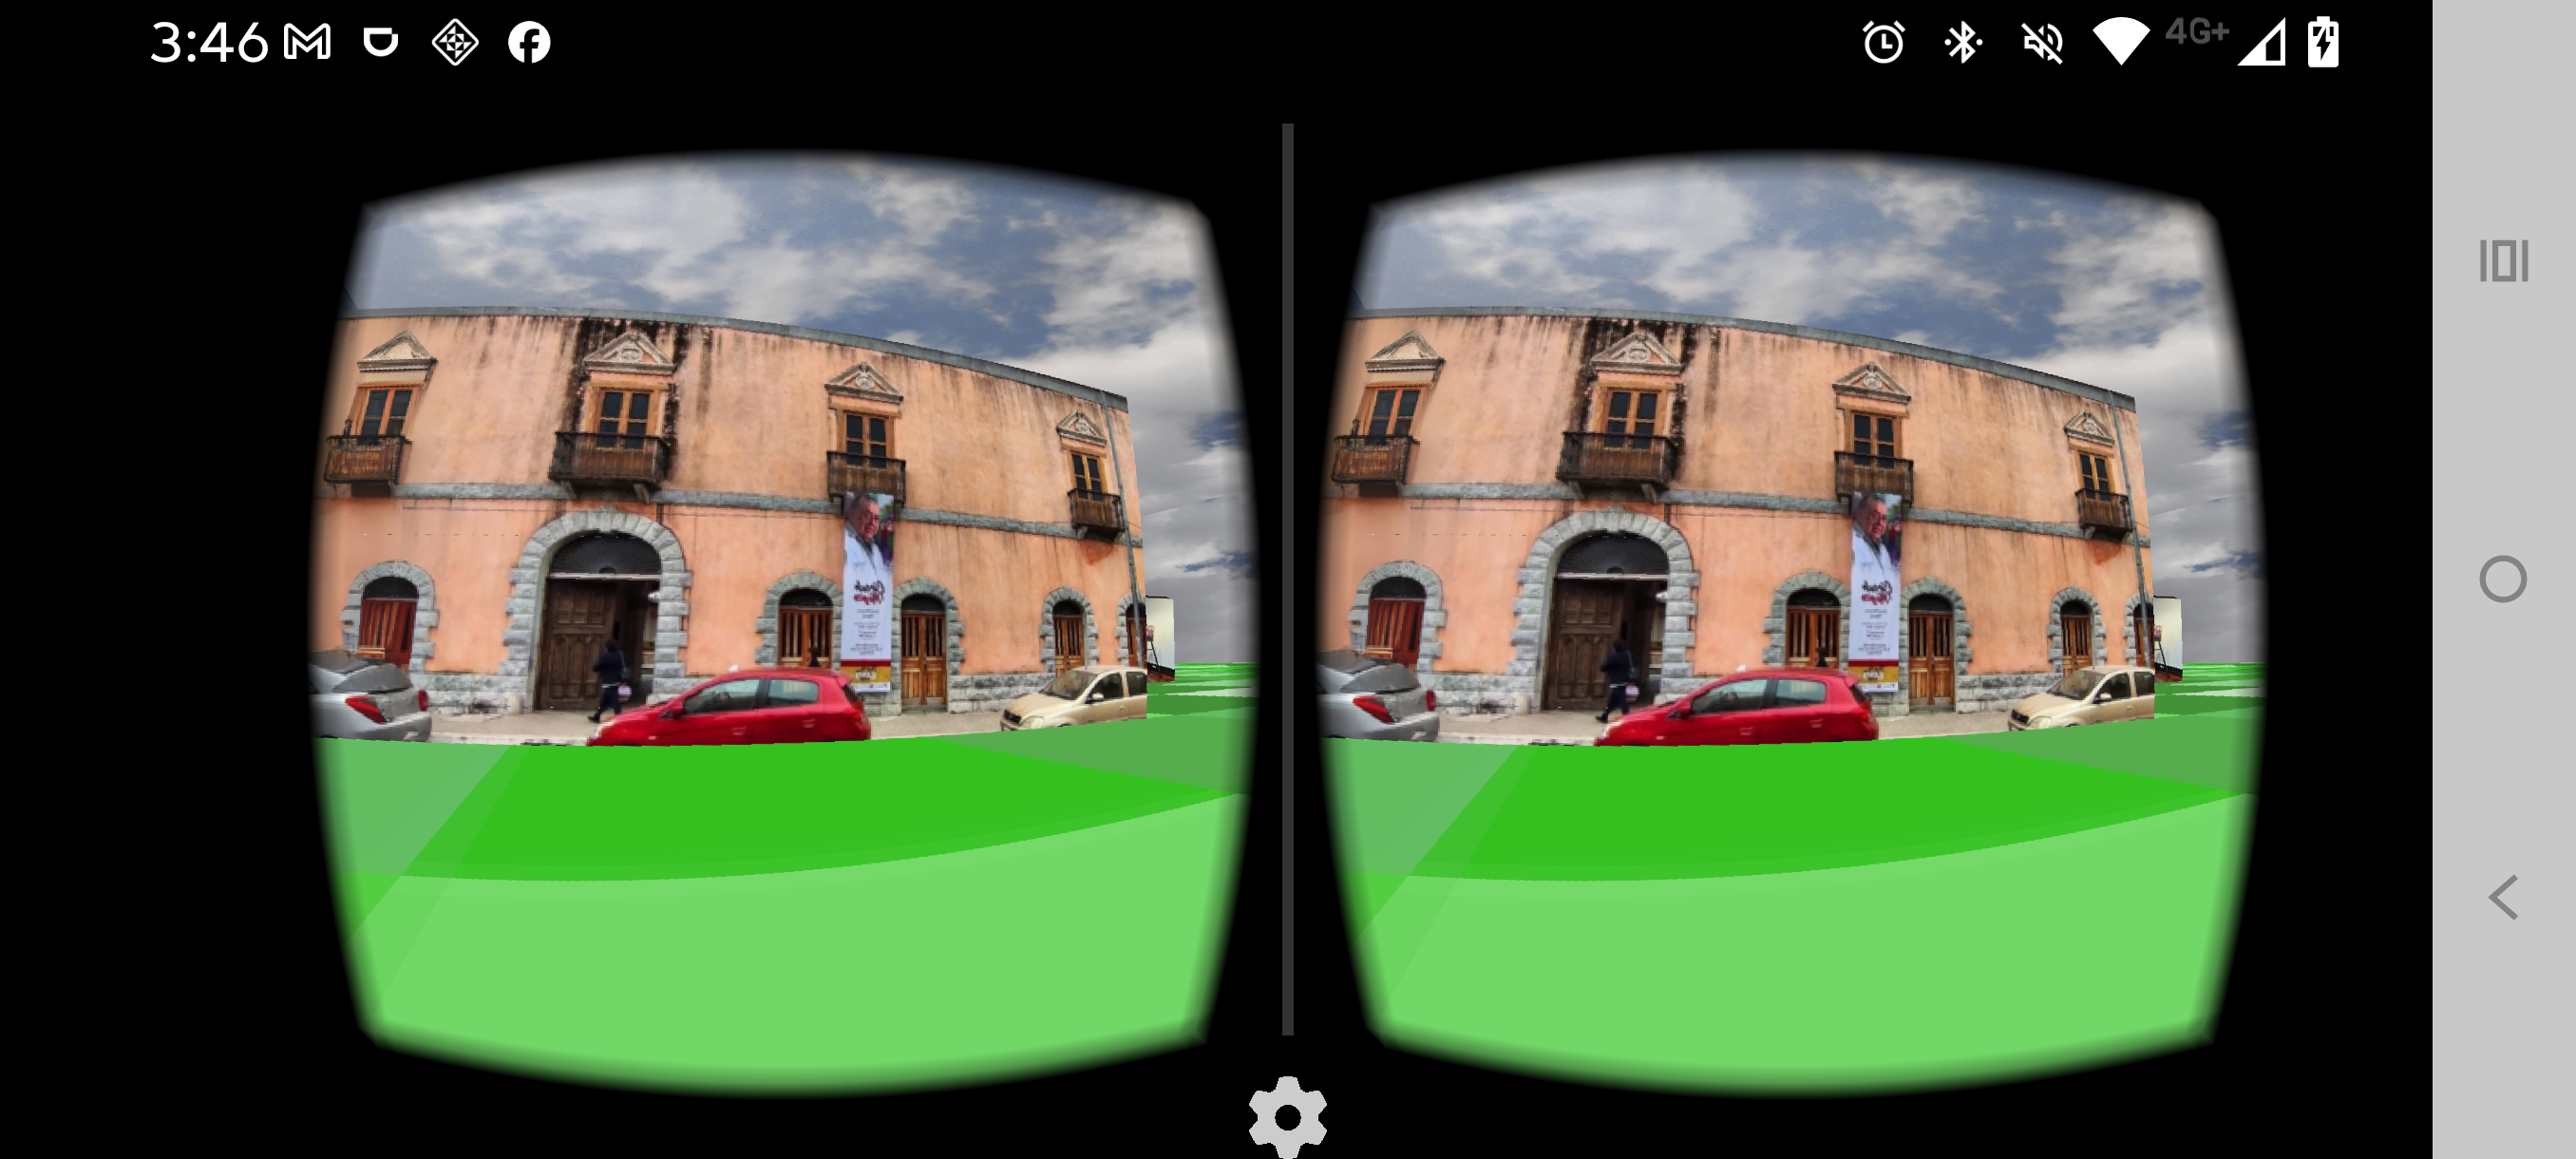
\includegraphics[width=0.45\linewidth]{2024_Pinacoteca_Virtual/Pinacoteca0} &
		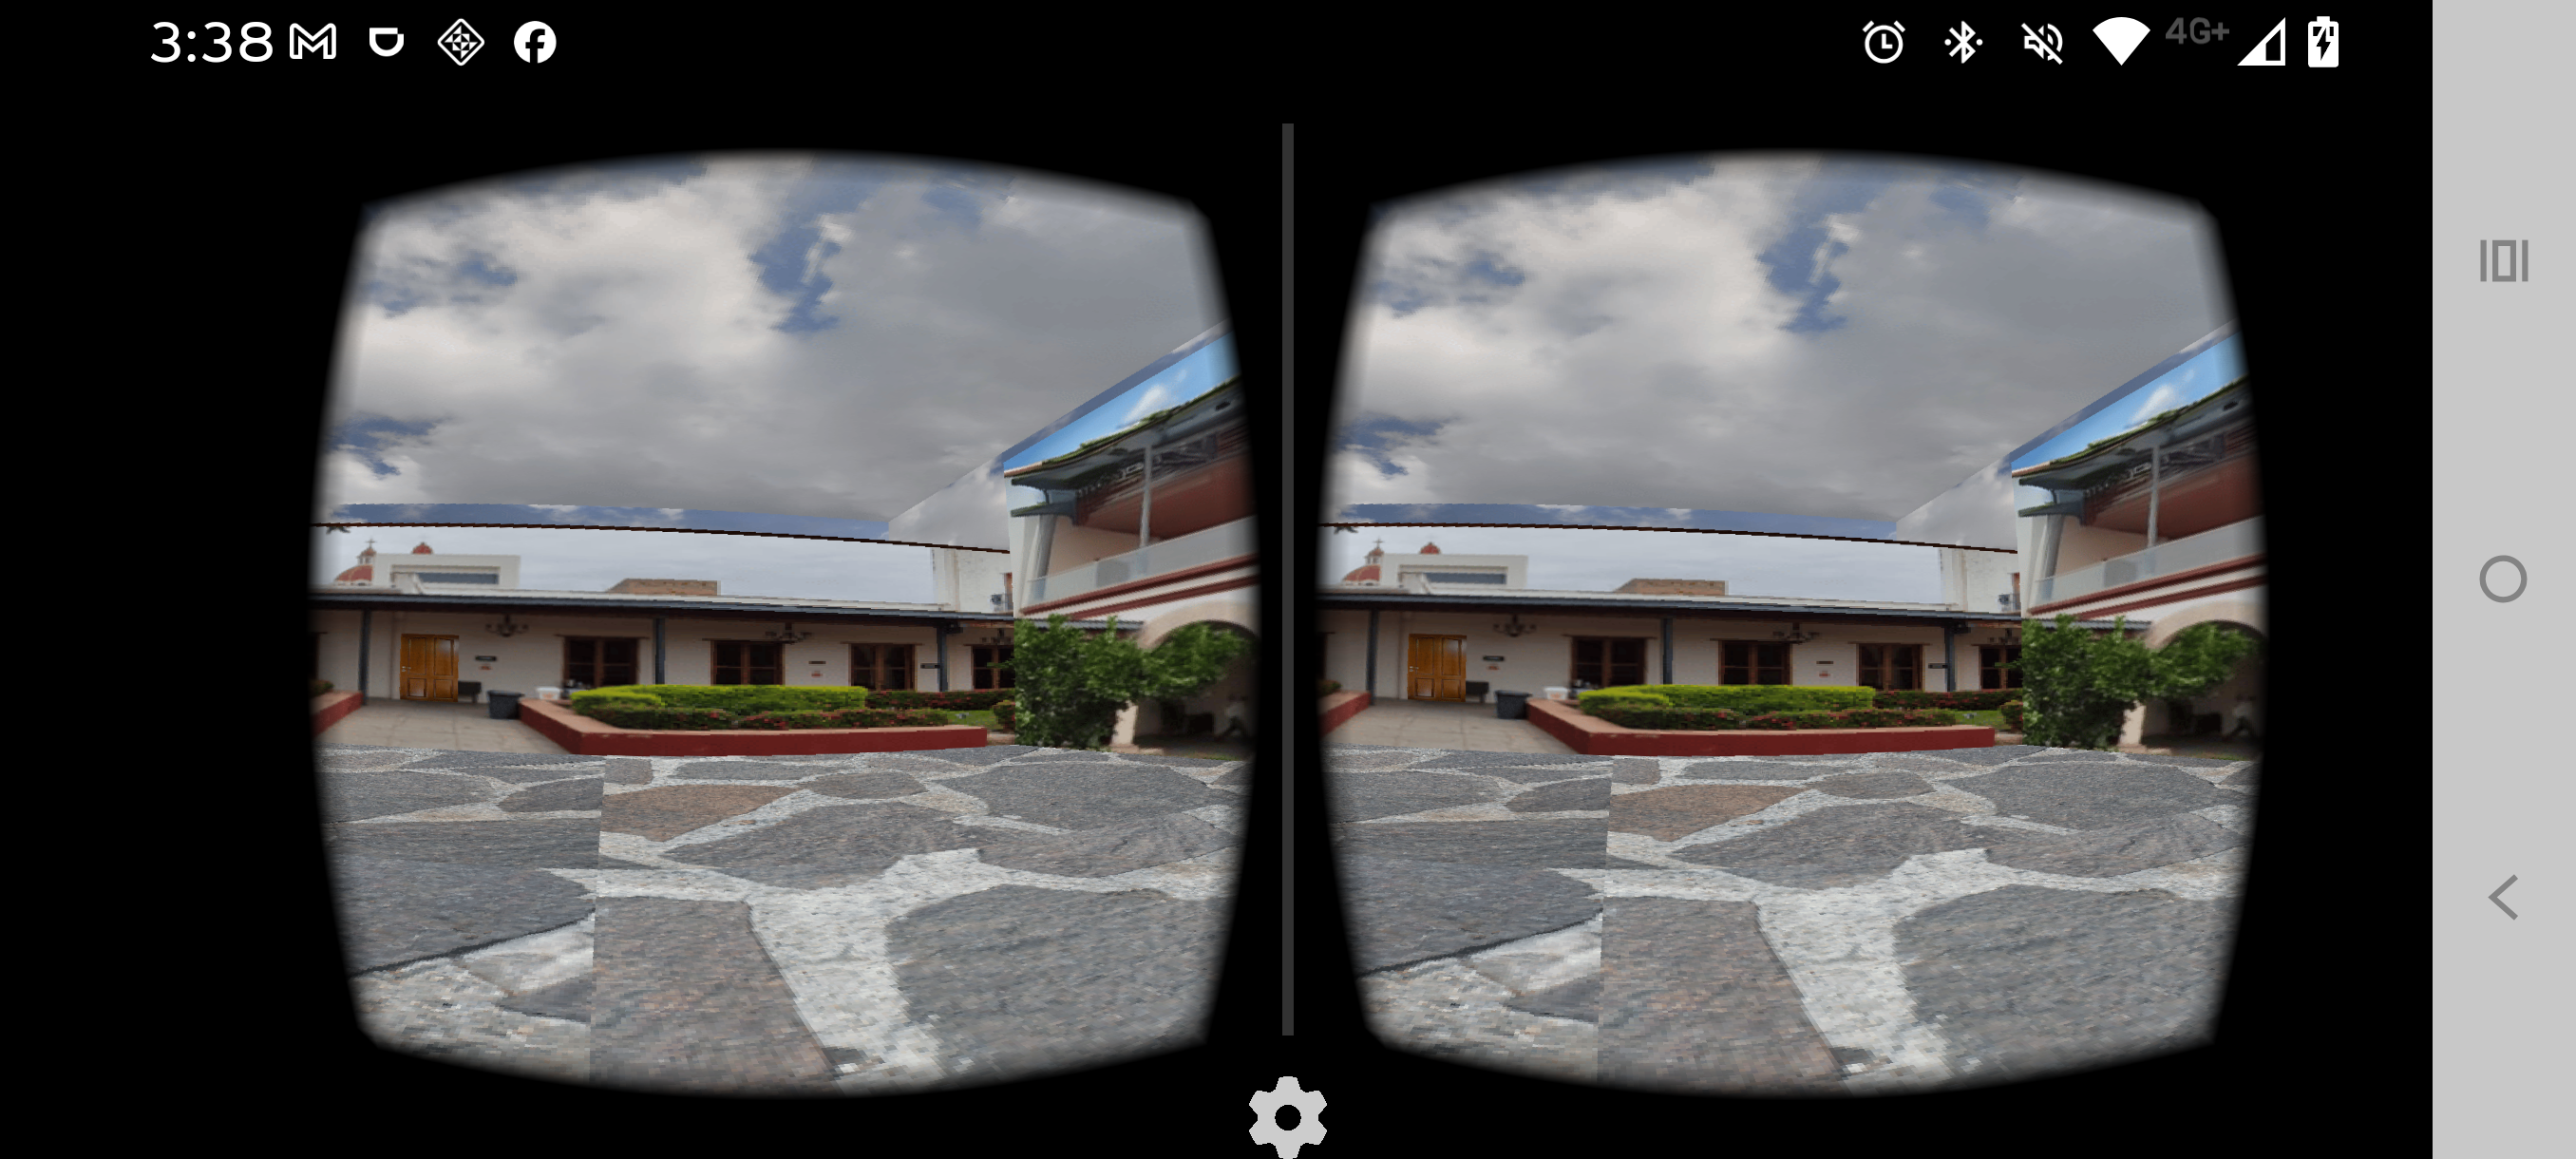
\includegraphics[width=0.45\linewidth]{2024_Pinacoteca_Virtual/Pinacoteca3} \\
		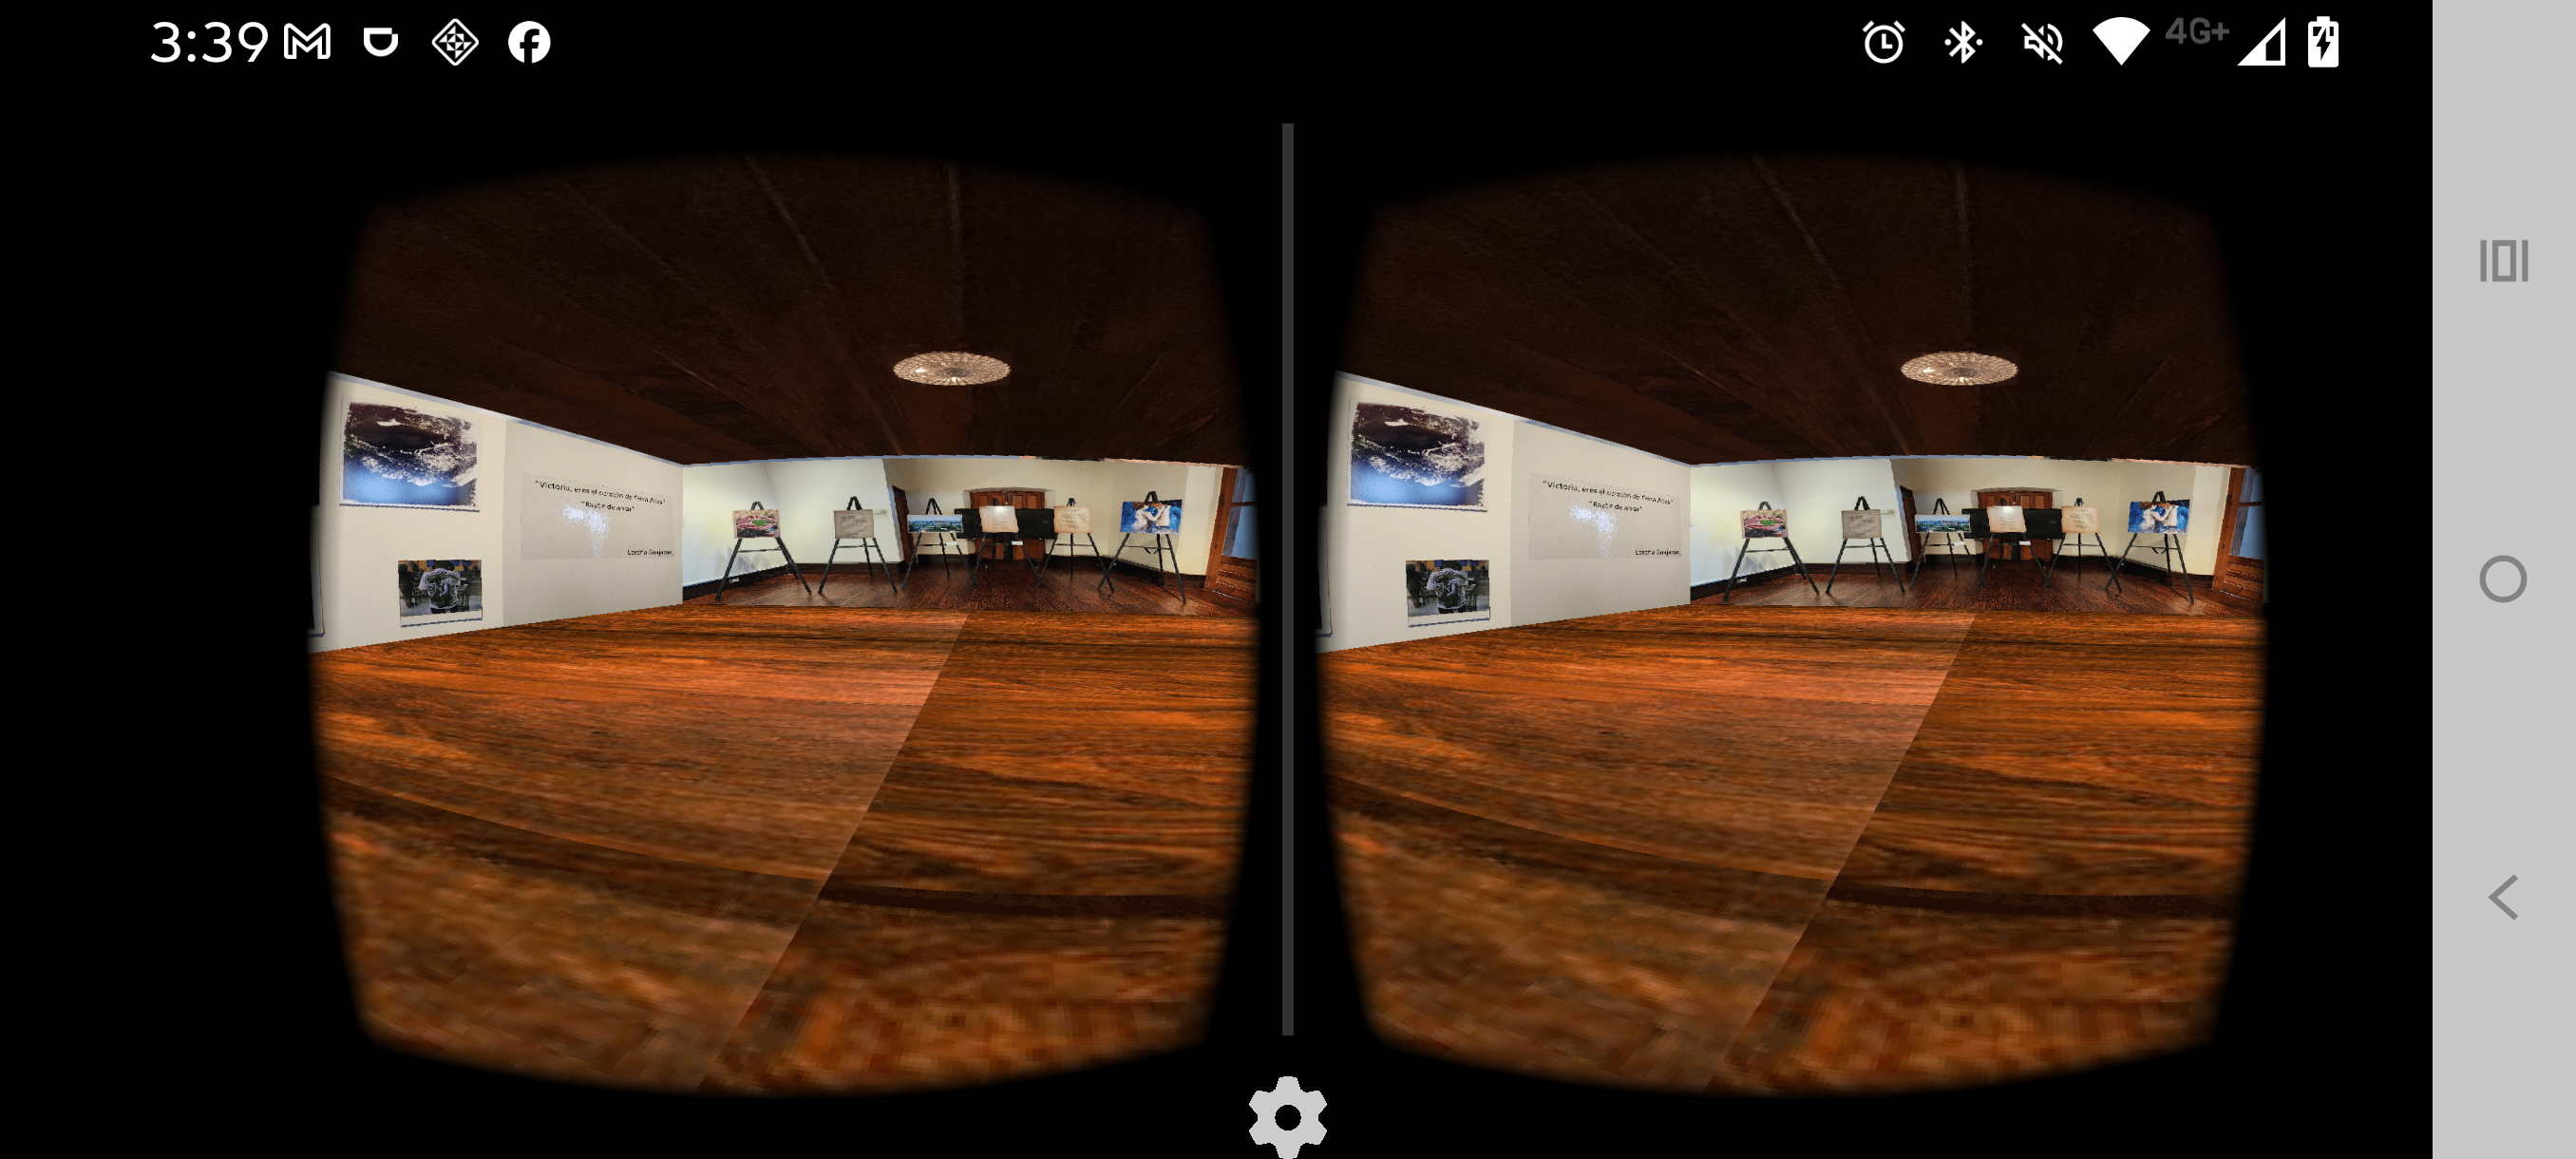
\includegraphics[width=0.45\linewidth]{2024_Pinacoteca_Virtual/Pinacoteca7} &
 		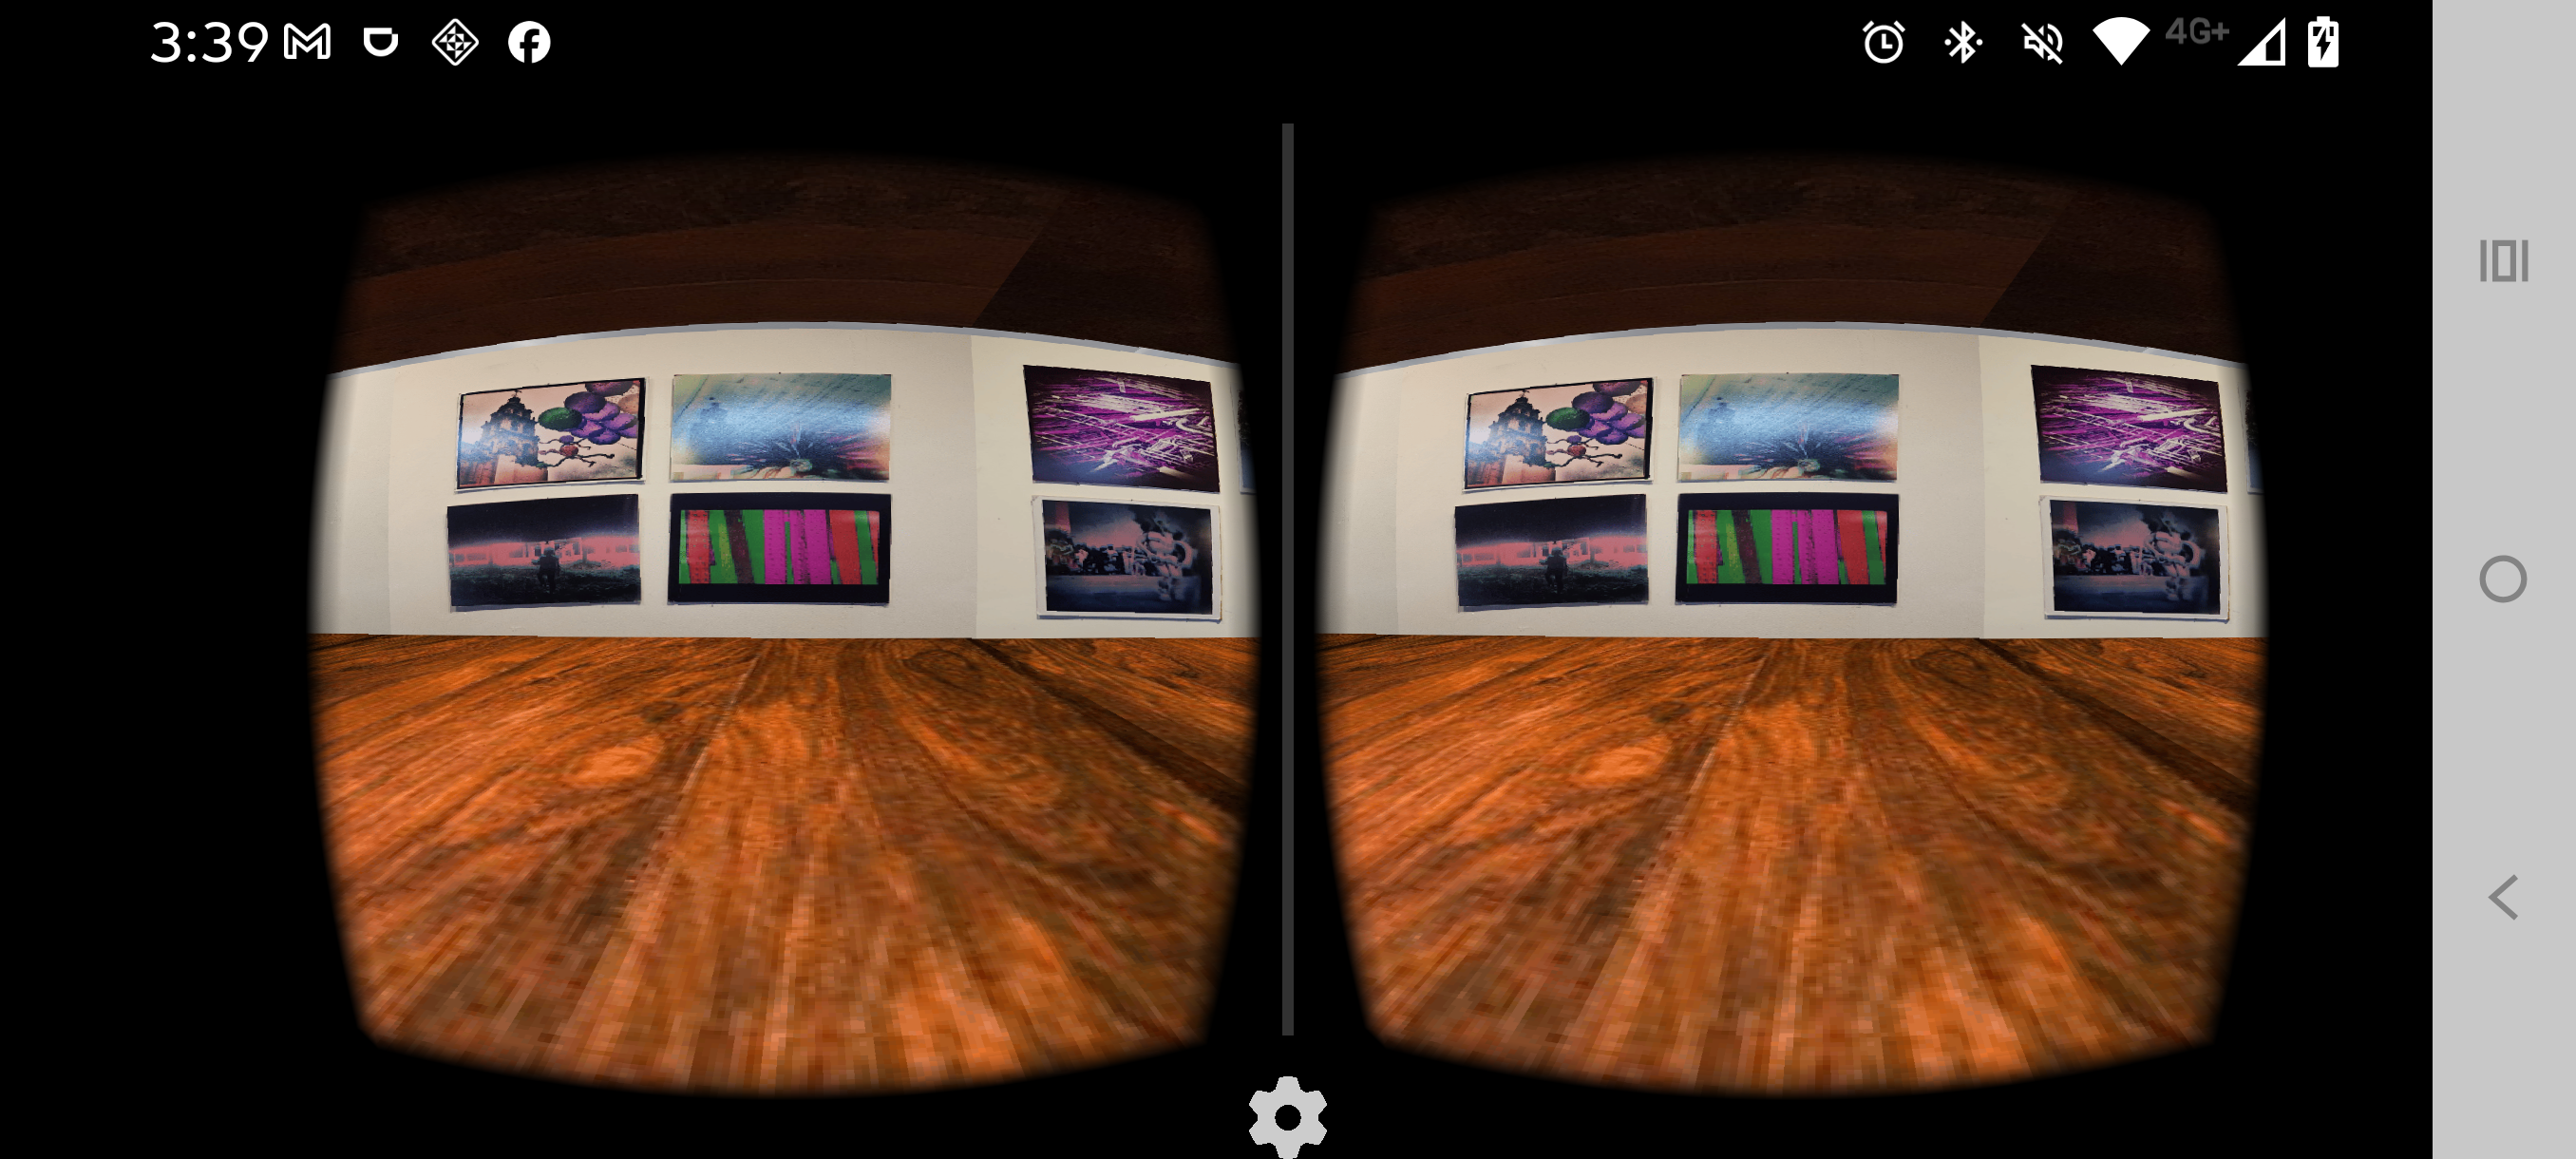
\includegraphics[width=0.45\linewidth]{2024_Pinacoteca_Virtual/Pinacoteca8} \\
	\end{tabular}
\end{center}



%\column{.5\linewidth}
%\begin{center}
	%\begin{tabular}{cccc}
	%	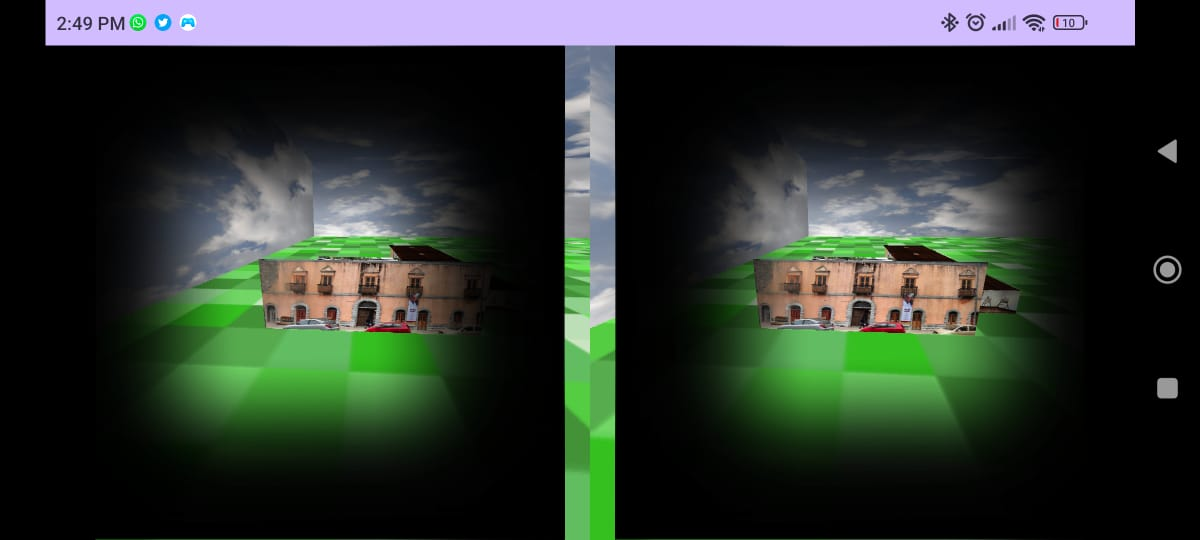
\includegraphics[width=0.40\linewidth]{2024_Pinacoteca_Virtual/PlanoGeneral.jpeg} &
 	%	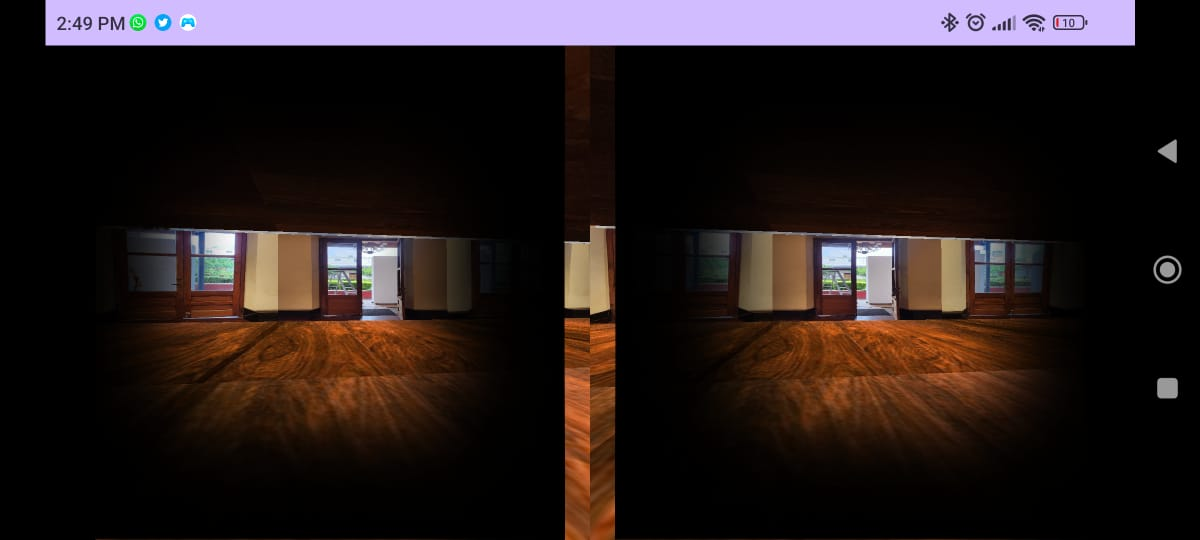
\includegraphics[width=0.40\linewidth]{2024_Pinacoteca_Virtual/Salida_SalonExhibiciones.jpeg} \\
%	\end{tabular}
%\end{center}


\end{columns}
\end{frame}




%\renewcommand{\EntradaBibtex}{PinacotecaVirtual_2024}
\renewcommand{\Folder}{2025_RecorridoVirtualCasaArte}
\renewcommand{\EntradaBibtex}{2025_RecorridoVirtualCasaArte}


\begin{frame}{\citetitle{\EntradaBibtex}$^*$ (1)}
\begin{block}{Motivación} 
\begin{itemize}
\item Se implementó una aplicación móvil para explorar de manera interactiva la case del Arte en Ciudad Victoria Tamaulipas. 
\end{itemize}
\end{block} 
\begin{center}
\includegraphics[width=0.38\linewidth]{\Folder/figs/CasaArte.jpg}
\end{center}
\footfullcite*{\EntradaBibtex}
\end{frame}


\begin{frame}{\citetitle{\EntradaBibtex} (2)}
%\begin{block}{Pantallas Principales} 

\begin{columns}
% Column 1
\column{.99\linewidth}



\begin{center}
	\begin{tabular}{cc}
		\includegraphics[width=0.45\linewidth]{\Folder/figs/CasaDelArte0} &
		\includegraphics[width=0.45\linewidth]{\Folder/figs/CasaDelArte2} \\
		\includegraphics[width=0.45\linewidth]{\Folder/figs/CasaDelArte7} &
 		\includegraphics[width=0.45\linewidth]{\Folder/figs/CasaDelArte6} \\
	\end{tabular}
\end{center}



%\column{.5\linewidth}
%\begin{center}
	%\begin{tabular}{cccc}
	%	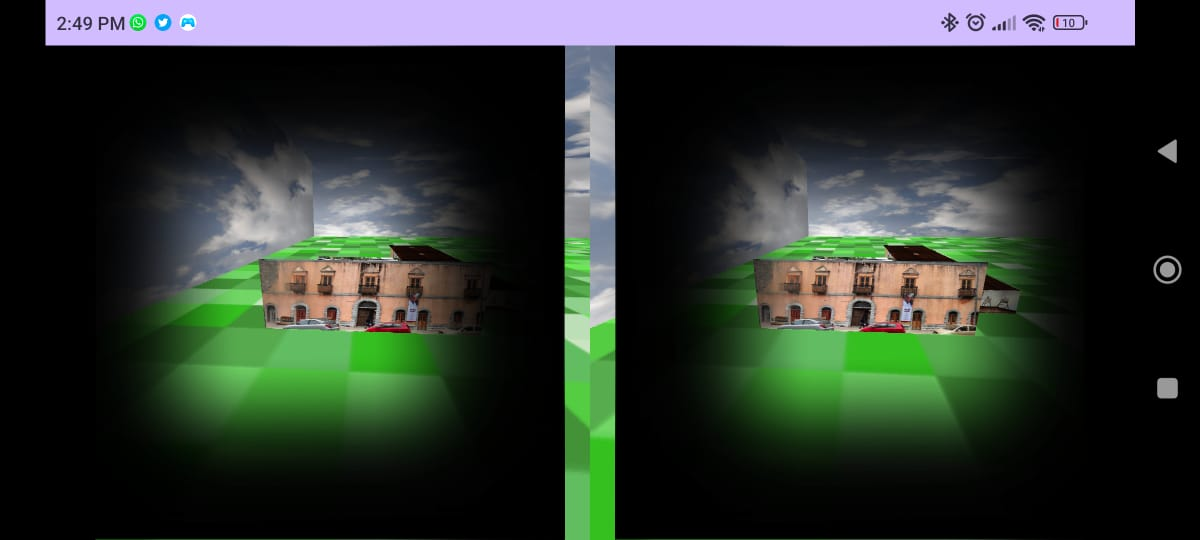
\includegraphics[width=0.40\linewidth]{2024_Pinacoteca_Virtual/PlanoGeneral.jpeg} &
 	%	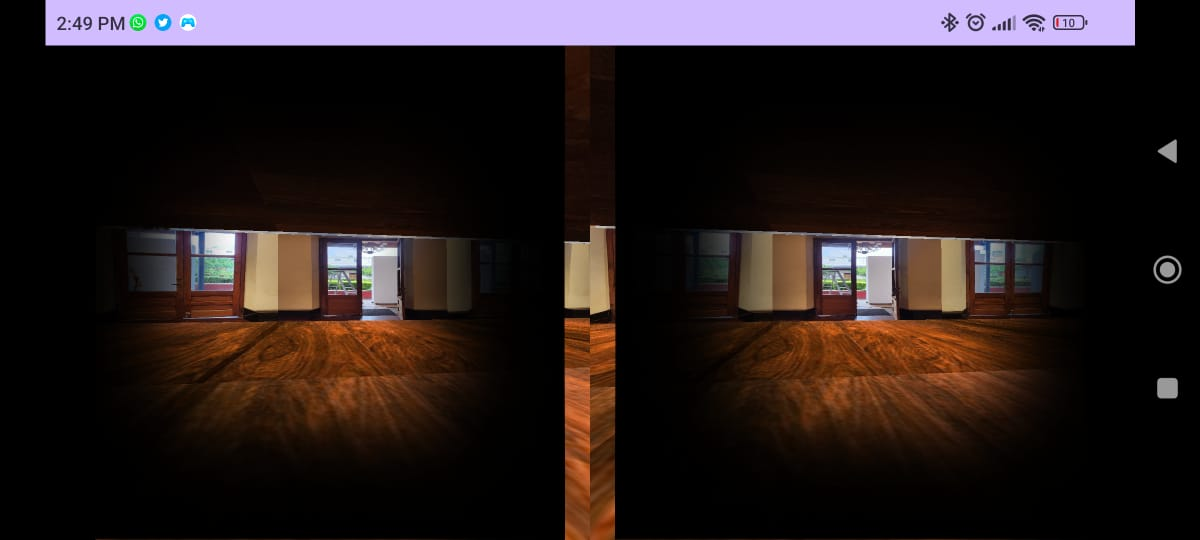
\includegraphics[width=0.40\linewidth]{2024_Pinacoteca_Virtual/Salida_SalonExhibiciones.jpeg} \\
%	\end{tabular}
%\end{center}


\end{columns}
\end{frame}




\renewcommand{\Folder}{2026_RecorridoTamux}
\renewcommand{\EntradaBibtex}{2026RecorridoVirtualTamux}
                              

\begin{frame}{\citetitle{\EntradaBibtex} \footnotemark[1] (1)}
\begin{columns}
	\begin{column}{0.40\textwidth}
		\begin{itemize}
			\item Modelado de una parte del Museo de Historia Natural de Tamaulipas TAMUX (Lobby y Sala 1).
			\item Mejoras por hacer: Agregar el exterior, pasillos del interior y el resto de las salas.  
		\end{itemize}
	\end{column}
	\begin{column}{0.30\textwidth}
		\begin{center}
			\includegraphics[width=0.98\textwidth]{\Folder/figs/ReF_Tamux1}
		\end{center}
	\end{column}
	\begin{column}{0.30\textwidth}
		 \begin{center}
		     \includegraphics[width=0.98\textwidth]{\Folder/figs/ReF_Tamux2}
		 \end{center}

	\end{column}
	
\end{columns}

%\end{block} 
\footnotetext[1]{\fullcite{\EntradaBibtex}}
\end{frame}


\begin{frame}{\citetitle{\EntradaBibtex}  (2)}
\begin{columns}
	\begin{column}{0.48\textwidth}
		\begin{center}
			\includegraphics[width=0.98\textwidth]{\Folder/figs/Tamux4}
		\end{center}
		 \begin{center}
		     \includegraphics[width=0.98\textwidth]{\Folder/figs/Tamux7}
		 \end{center}
	\end{column}
	\begin{column}{0.48\textwidth}
		\begin{center}
			\includegraphics[width=0.98\textwidth]{\Folder/figs/Tamux0}
		\end{center}
		 \begin{center}
		     \includegraphics[width=0.98\textwidth]{\Folder/figs/Tamux2}
		 \end{center}

	\end{column}
	
\end{columns}

%\end{block} 
%\footnotetext[1]{\fullcite{\EntradaBibtex}}
\end{frame}




\section[CP1]{Conclusiones }
\begin{frame}{Conclusi\'on y Áreas de Oportunidad}
En esta presentacion:
\begin{itemize}
\item se presentaron conceptos relacionados con la RV. 
\item se describen las herramientas requeridas para interactuar con los demos realizados. 
\item se describen los demos implementados. Es posible que os asistentes interactúen con los demos presentados si se solicita extender esta presentación de manera presencial.
\end{itemize}
Areas de oportunidad:
\begin{itemize}
\item Abiertos a propuestas de proyectos y/o exploracion de plataformas alternas.
\item Posibilidades de proyectos bajo financiamiento externo en multiples aplicaciones.
\end{itemize}

\end{frame}



\end{document}

